\documentclass[12pt]{article}

\usepackage{fullpage}
\usepackage{graphicx}
\usepackage{graphics}
\usepackage{mdwlist}
\usepackage{float}

% christos: these look closer to NSF specs\dots
\setlength{\oddsidemargin}{0.0in}
\setlength{\evensidemargin}{0.0in}
\setlength{\textwidth}{6.5in}
\setlength{\headheight}{0.0in}
\setlength{\topmargin}{0.0in}
% \setlength{\textheight}{9.0in}
\setlength{\textheight}{9in}
\addtolength{\textheight}{-\topmargin}
\addtolength{\textheight}{-\headheight}
\addtolength{\textheight}{-\headsep}
\addtolength{\textheight}{-\footskip}



\begin{document}

\newcommand{\beq}{\begin{equation}}
\newcommand{\eeq}{\end{equation}}
\newcommand{\bit}{\begin{itemize*}}
\newcommand{\eit}{\end{itemize*}}
\newcommand{\goal}[1]{ {\noindent {$\Rightarrow$} \em {#1} } }
\newcommand{\hide}[1]{}
\newcommand{\comment}[1]{ {\footnotesize {#1} } }
\newtheorem{lemma}{Lemma}
\newtheorem{theorem}{Theorem}
\newtheorem{proof}{Proof}
\newtheorem{defn}{Definition}
\newtheorem{algo}{Algorithm}
\newtheorem{observation}{Observation}

\title{Graph Mining Using SQL}


\author{ 
	{\em Ye Zhou} \\
	    School of Computer Science \\
	    CMU\\
	    {\tt yezhou@cs.cmu.edu}
	 \and
	 {\em Jin Hu} \\
	     School of Computer Science \\
	    CMU\\
	     {\tt jinh@cs.cmu.edu}
}


\maketitle
\begin{abstract}
    In this project, we investigated the possibility of using only SQL to do graph manipulations
on {\em graphMiner}. 
{\em graphMiner} contains generic methods for RDBMS manipulations and some graph mining algorithms such as PageRank, Degree Distribution, Weak Connected Components, etc. Many useful properties of graphs can be found using these methods. {\em graphMiner} is based on Python, Postgres Database and SQL. Python provides basic control and logic as well as file operations, while all the important calculations are done through SQL on Postgres Database. 
We also implemented kcore algorithm within the framework, which gives useful information of the importance of nodes in the graph.
We created unit tests on kcore and other algorithms in the system to test their functionality and correctness as well as to gain better understanding of these methods. 
For real world testing, we also ran kcore and other algorithms in the framework on 20 realworld datasets. We found some interesting properties of these datasets and explained them with the findings from the results of these graph mining algorithms.

\end{abstract}

\section{Introduction}
    \label{sec:intro}
    % {\em
% \bit
% \item
% what is the problem
% \item
% what are the applications
% \eit
% }
{\small \em Specify the problem; Give the motivation; 
List your main contributions}

The problem we are trying to solve is: Given a graph of source-destination pairs on disk, we try to use only SQL to implement basic matrix and vector operations, which make it possible to handle more complex graph manipulations. We will then be able to implement algorithms like PageRank and Degree distribution without the need of an additional language.

The motivation is that we can use only SQL and do not need to depend on other languages. With SQL we can enjoy the benefits of various features of databases and become more effcient in implementing and testing some of the algorithms without the worries like data structure, memory optimization, file IO, etc.

Doing graph mining with SQL is an important method for all scales, research or industry use, as database provides easier interface to scale and deploy. And graph manipulation and mining has many real world applications and is a very important topic. Thus a convenient way of implementing graph manipulation algorithms are highly desired.

The contributions of this project are the following:
\bit
\item Our implemented {\em K-core Decomposition} is fast and uses only SQL to do the calculations. Python only works as 
some basic loop control and input output format handling.
\item We tested various graph handling algorithm on unit tests and some real world datasets.
\eit


\section{Survey}
    \label{sec:survey}
    Next we list the papers that each member read,
along with their summary and critique.

\subsection{Papers read by Ye Zhou}
The first paper was the Pegasus paper by U Kang
\begin{itemize*}
\item {\em Main idea}: 
      When graph data grows larger and larger, using traditional graph mining algorithms is difficult to deal with trend. In order to solve the graph 
      mining problems with several Petabytes data, Pegasus is the first such library, impelemted on the top of Hadoop platform. In the paper, first they 
      try to find out the common operation, which is the matrix-vector multipilication, underlying several primitive graph mining operations. They call it 
      GIM-V. As GIM-V is so important, they successfully proposed several optimizations, and got more than 5 times faster performance. They also took real 
      big data graph into Pegasus to get the mining result, which revealed important patterns. This showed the succuess of Pegasus with large data graph 
      mininig as the graph data they used had never been studied before.
\item {\em Use for our project}:
      It showed that with large data, we always have new problems using traditional graph mining methods. It is really hard to say that with SQL, we can 
      do enough with graph mining now, as SQL is based on RMDB. But with more and more new mature products/framework like hive, pig, shark which support 
      traditional SQL operations on big data and No-SQL database, we can do more with SQL. 
\item {\em Shortcomings}:
      PEGASUS focus on large graph querying/mining and most of the job was focused on how to compute fast, but it ignored the storage part which can also 
      take effect to improve the performance like indexing. In addition, PEGASUS essentially perform node/vertex-centralized computation but cannot 
      supports edge-centralized processing like induced subgraphs. Finally, hadoop is not so efficient for iterative calculation, as everytime it needs to 
      write output data to hard disk. Spark has better performance as it output its intermediate data in memory and can even cahche the data in memory.
\end{itemize*}

\subsection{Papers read by Ye Zhou}
The second paper was the Spectral Analysis for Billion-Scale Graphs paper by U Kang
\begin{itemize*}
\item {\em Main idea}: 
      The paper proposed HEIGEN algorithm which is designed to be accurate, efficient to run on highly scalable hadoop environment and solve the problems 
      that will calculate out the spectral value. The paper first showed specific observation using HEIGEN with real world data on billion-scale graphs,
      focusing on structural property of networks: spotting near-cliques and finding triangles. Then the author explained that the alternatives for computing
      the eigenvalues of symmetric matrix including Power Method, Simultaneous iteration and Lanczos-NO are not suitable for big data on mapreduce. So the author
      described the algorithm for computing the top K eigenvectors and eigenvalues with four speficic fields improvement: Careful Algorithm Choice, selective 
      parallelization, blocking and skewness exploiting. Finally it turned out that performance improved in both scalabitily and skewed matrix data, compared with 
      HEIGEN-PLAIN.
\item {\em Use for our project}:
      Largely based on mapreduce, HEIGEN is a totally new algorithm. What we can learn is that with massive data, we can change the former way of thinking for graph mining,
      so that we can largely improve the performance without SQL. And also, with the infrastructure of hadoop, and the way map/reduce reading data, we can do modification
      to use the advantages to get even better performance.
\item {\em Shortcomings}:
      Highly based on map/reduce architecture also brings lots of problems that hadoop has. Such as the job schedualing and data shuffling. As the matrix operation needs to
      read large amount of data, and for iterative calculation, spark is a better choice as everything is in memory. 
\end{itemize*}

\subsection{Papers read by Ye Zhou}
The third paper was the Unifying Guil-by-Association Approaches paper by Koutra
\begin{itemize*}
\item {\em Main idea}: 
      The paper mainly proposed FaBP, which is a Fast Belief Propagation algorithm on Hadoop. It first compare and contrast several very successful, guilt-by-association methods:
      Random Walk with Restarts, Semi-Supervised Learning and Belief Propagation. The author showed that these three methods are closedly related but not identical. Then he proposed
      the algorithm FaBP, showed the experiments result. It turned out that the accuracy keeps the same or even better with the traditional BP, but the performance is twice better.
      It also has convergence guarantee. It is even sensitive to the "about-half" homophily factor, as long as the latter is within the convergence bounds. It also scales linearly
      on the number of edges. 
\item {\em Use for our project}:
      Learn the way using hadoop to impelment the algorithm for machine learning. 
\item {\em Shortcomings}:
      Again it is based on Hadoop, the performance for iterative calculation is not so good compared with spark. And BP algorithm is not so efficient when dealing with graph which
      has circle. And the convergence is limited due to specific requirement.
\end{itemize*}

\subsection{Papers read by Jin Hu}
The first paper was the GBASE paper by U Kang
\begin{itemize*}
\item {\em Main idea}: The paper introduces a general graph management system GBase for large scale graph storage and computation.
\item {\em The main contribution of the paper:}:
      GBase uses "compressed block encoding" method to make graph storage more efficiently.
    For graph indexing, the paper succeeds in handling multiple type of queries on a large graph instead of a specific type and is suitable for distributed environment. By supporting homogeneous block level indexing and being flexible in both edge and node centralized computing, GBase has better properties than similar distributed systems.
    The framework the paper proposes also supported both graph-level and node-level queries, making it applicable to various applications.
    GBase partitions data in two dimensions to better use the block and community-like properties of real-world graphs,
    which gives it advantage over either row-oriented or column-oriented storages.
\item {\em Limitations}:
      The paper's indexing method handles large graphs successfully, but its property compared to frequent subgraph
    or significant graph pattern methods are not shown in the experiment. Optional indexing methods may be added to
    the system.
\end{itemize*}

\subsection{Papers read by Jin Hu}
The second paper was by Danai Koutra
\begin{itemize*}
\item {\em Main idea}: The paper does the comparison among some of the most popular guilt-by-association method.
\item {\em The main contribution of the paper:}:
      The paper manages to prove that all methods result in a similar matrix inversion problem. In addition, the paper proposes a fast and accurate BP algorithm. In theory, the paper finds that RWR(Personalized Random Walk with Restats), SSL(Semi-Supervised Learning) and BP(Belief Propagation) are closely related, but not the same. RWR and SSL are not heterophily, but BP is heterophily. All three methods are scalable. RWR and SSL have convergence while BP is unknown. The proposed FABP method has nice property with all these perspectives. FABP is an approximation of standard BP, but FABP is significantly faster based on the experiment and guarantees convergence, which makes it better than BP. The experiments also verify the paper's ideas. The author tested the theory and the properties of the proposed FABP method in terms of accuracy, convergence, sensitivity to parameters and scalability.
\end{itemize*}

\subsection{Papers read by Jin Hu}
The third paper was by Ignacio Alvarez-Hamelin
\begin{itemize*}
\item {\em Main idea}: The paper introduces K-core decomposition and its application in the visulization of large scale networks.
\item {\em The main contribution of the paper:}:
	K-core decomposition can find subgraphs which all of the nodes in the subgraph have degrees higher than k after removing nodes with lower coreness. This method can find the subgraphs which are more closely connected and achieves "clustering" in large graphs.
      As K-core decomposition can produce two-dimensional layout of large scale networks with their important topological and hierarchical properties, the paper takes advantage of the K-core algorithm to allow visulization of network and offer features like fingerprint identification and general analysis assistance. The visualization algorithm has linear running time proportional to the size of the network, making it well scalable for large networks. In addition, the algorithm offers 2D representation of networks which makes information visualization more accessible than other representations and the parameters of the algorithm are universally defined, which makes it suitable for all types of networks.
\item {\em Limitations}:
      The proposed visualization algorithm still utilizes certain parameters to identify the properties of the network, which involves considerable human interactions and prior expemental knowledge. Self adjusting parameters might be a huge improvement and can be an interesting topic to follow.
\end{itemize*}

$\ldots$



\section{Proposed Method}
    \label{sec:proposed}
    We implemented K-core using SQL following the Batagelj and Zaversnik k-core variation. We recursively prune the nodes and edges in the graph with degree less than k to finally arrive at points of degree greater than or equal to k. 





\section{Experiments}
    \label{sec:experiments}
    
We implemented kcores method
and tested other algorithms that are already implemented in the system with unit tests and 20 realworld datasets described in the appendix.

Figures below give the degree distribution and pagerank result of 20 datasets. We can find that the degree distribution and pagerank results are consistent with the power law as nodes or pages with higher degree or rank have a small number while nodes or pages with lower degree or rank have a large number.
You can also find the detailed results in the output folder, which contains csv files for the results of belief propagation, connected components, node degrees, degree distribution, eigen values, k-core connected components, pagerank results, radius, etc. More detailed analysis and anomaly discussion are discussed below.


\begin{figure}[H]
\begin{center}
\begin{tabular}{cc}
     % uncomment the next lines, and give the right ps files
     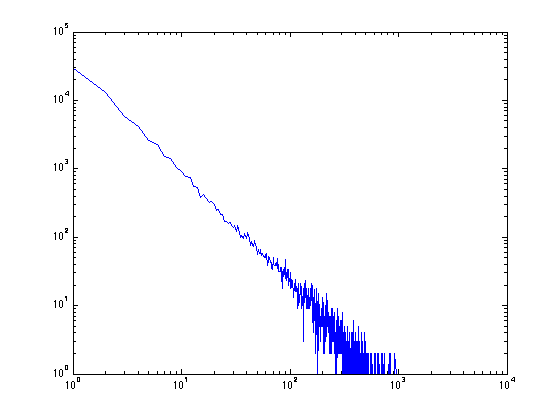
\includegraphics[width=0.3\textwidth]{FIG/soc-degreedist.png} &
     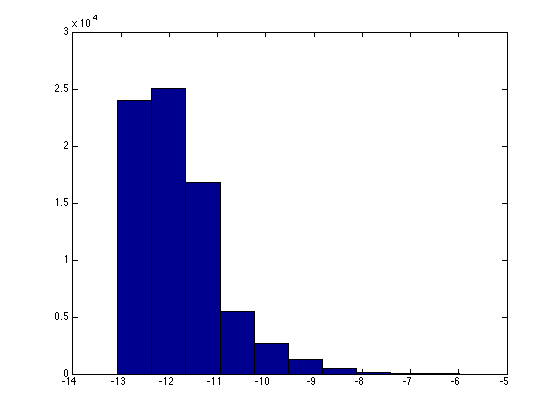
\includegraphics[width=0.3\textwidth]{FIG/soc-pagerank.png} \\
\end{tabular}
\caption{Degree Distribution(a) and PageRank(b) for Dataset SOC-Epinions1}

\begin{tabular}{cc}
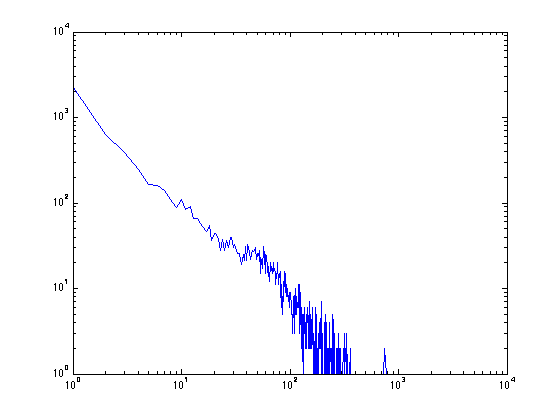
\includegraphics[width=0.3\textwidth]{FIG/wiki-degreedist.png} &
     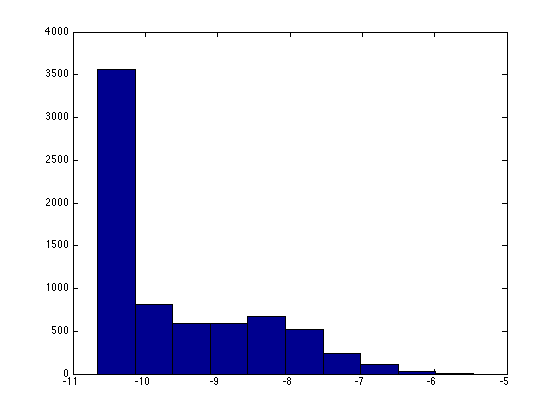
\includegraphics[width=0.3\textwidth]{FIG/wiki-pagerank.png} \\

     %\psfig{figure=FIG/plot.ps,width=2in} \\
     % \psfig{figure=FIG/data.ps,width=2in} &
     % \psfig{figure=FIG/plot.ps,width=2in} \\
    (a) & (b)
\end{tabular}
\caption{Degree Distribution(a) and PageRank(b) for Dataset wiki-Vote}

\end{center}
\end{figure}

The figures below also include the degree distribution, connected components, k=5 cores algorithm results on the 5 unit tests.
As the unit tests are small, there is no nodes in the tests that satisfy k=5 cores, so the output result for these 5 
unit tests are empty. 
However, you can find the node id, component id pairs in the stdout output from console or in the kcorecomponent.csv file, which shows that the k-core
algorithm works as it claims to find correct coreness subgraphs.

\begin{figure}[H]
\begin{center}
\begin{tabular}{cc}
     % uncomment the next lines, and give the right ps files
     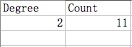
\includegraphics[width=0.3\textwidth]{FIG/1dd.jpg} &
     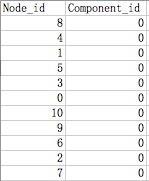
\includegraphics[width=0.3\textwidth]{FIG/1cc.jpg} \\
\end{tabular}
\caption{Degree Distribution(a), connected components(b) for Dataset1}
\end{center}
\end{figure}

\begin{figure}[H]
\begin{center}
\begin{tabular}{cc}
     % uncomment the next lines, and give the right ps files
     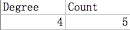
\includegraphics[width=0.3\textwidth]{FIG/2dd.jpg} &
     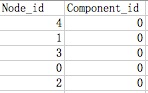
\includegraphics[width=0.3\textwidth]{FIG/2cc.jpg} \\
\end{tabular}
\caption{Degree Distribution(a), connected components(b) for Dataset2}
\end{center}
\end{figure}

\begin{figure}[H]
\begin{center}
\begin{tabular}{cc}
     % uncomment the next lines, and give the right ps files
     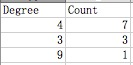
\includegraphics[width=0.3\textwidth]{FIG/3dd.jpg} &
     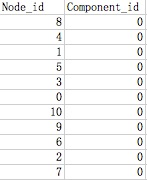
\includegraphics[width=0.3\textwidth]{FIG/3cc.jpg} \\
\end{tabular}
\caption{Degree Distribution(a), connected components(b) for Dataset3}
\end{center}
\end{figure}

\begin{figure}[H]
\begin{center}
\begin{tabular}{cc}
     % uncomment the next lines, and give the right ps files
     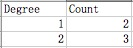
\includegraphics[width=0.3\textwidth]{FIG/4dd.jpg} &
     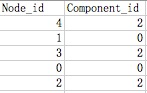
\includegraphics[width=0.3\textwidth]{FIG/4cc.jpg} \\
\end{tabular}
\caption{Degree Distribution(a), connected components(b) for Dataset4}
\end{center}
\end{figure}

\begin{figure}[H]
\begin{center}
\begin{tabular}{cc}
     % uncomment the next lines, and give the right ps files
     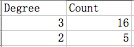
\includegraphics[width=0.3\textwidth]{FIG/5dd.jpg} &
     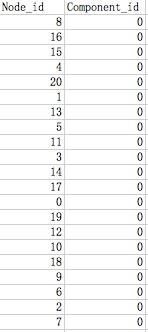
\includegraphics[width=0.3\textwidth]{FIG/5cc.jpg} \\
\end{tabular}
\caption{Degree Distribution(a) connected components(b) for Dataset5}
\end{center}
\end{figure}


We build index for algorithms Degree Distribution, K-core, Pagerank, Connected Components, All Radius, Eigen Value Computation on ten datasets:as-skitter.ungraph-75000, ca-AstroPh, cit-HepPh, cit-HepTh, com-amazon.ungraph-75000, com-dblp.ungraph-75000, email-Enron.ungraph, email-EuAll,p2p-Gnutella31, soc-Slashdot0811-75000.

We first conducted some simple tests to make sure that creating index can lead to performance improvement.
For example, 
Degree Distribution:(no index on node degree), run time is 147.476911545
Degree Distribution:(index on node degree (in degree, out degree)), run time is 346.571922302
From the experiment, create index does consume system resources and it will make performance worse in general if we
created index and used it only once.
However, 
Degree Distribution:(no index on node degree)(run 10 times), run time is 2091.14193916,
Degree Distribution:(index on node degree (in degree, out degree))(run 10 times, 1 time create index), run time is 1351.35889053.
From the experiment, create index will improve performance in general if we created index and used it later a lot.
Also, for a certain algorithm, create index for some tables like GMNODES are expensive, but if re run all the algorithms,or use the algorithm multiple times, then the cost of creating index on tables like GMNODES will be worth the effort.

This is the general intuitive for us to choose on which table and which column to create index and avoid some unnecessay tests.

We compared building index for different tables on different columns for each algorithm and get the following figures below. 

\begin{figure}[H]
\begin{center}
\begin{tabular}{cc}
     % uncomment the next lines, and give the right ps files
     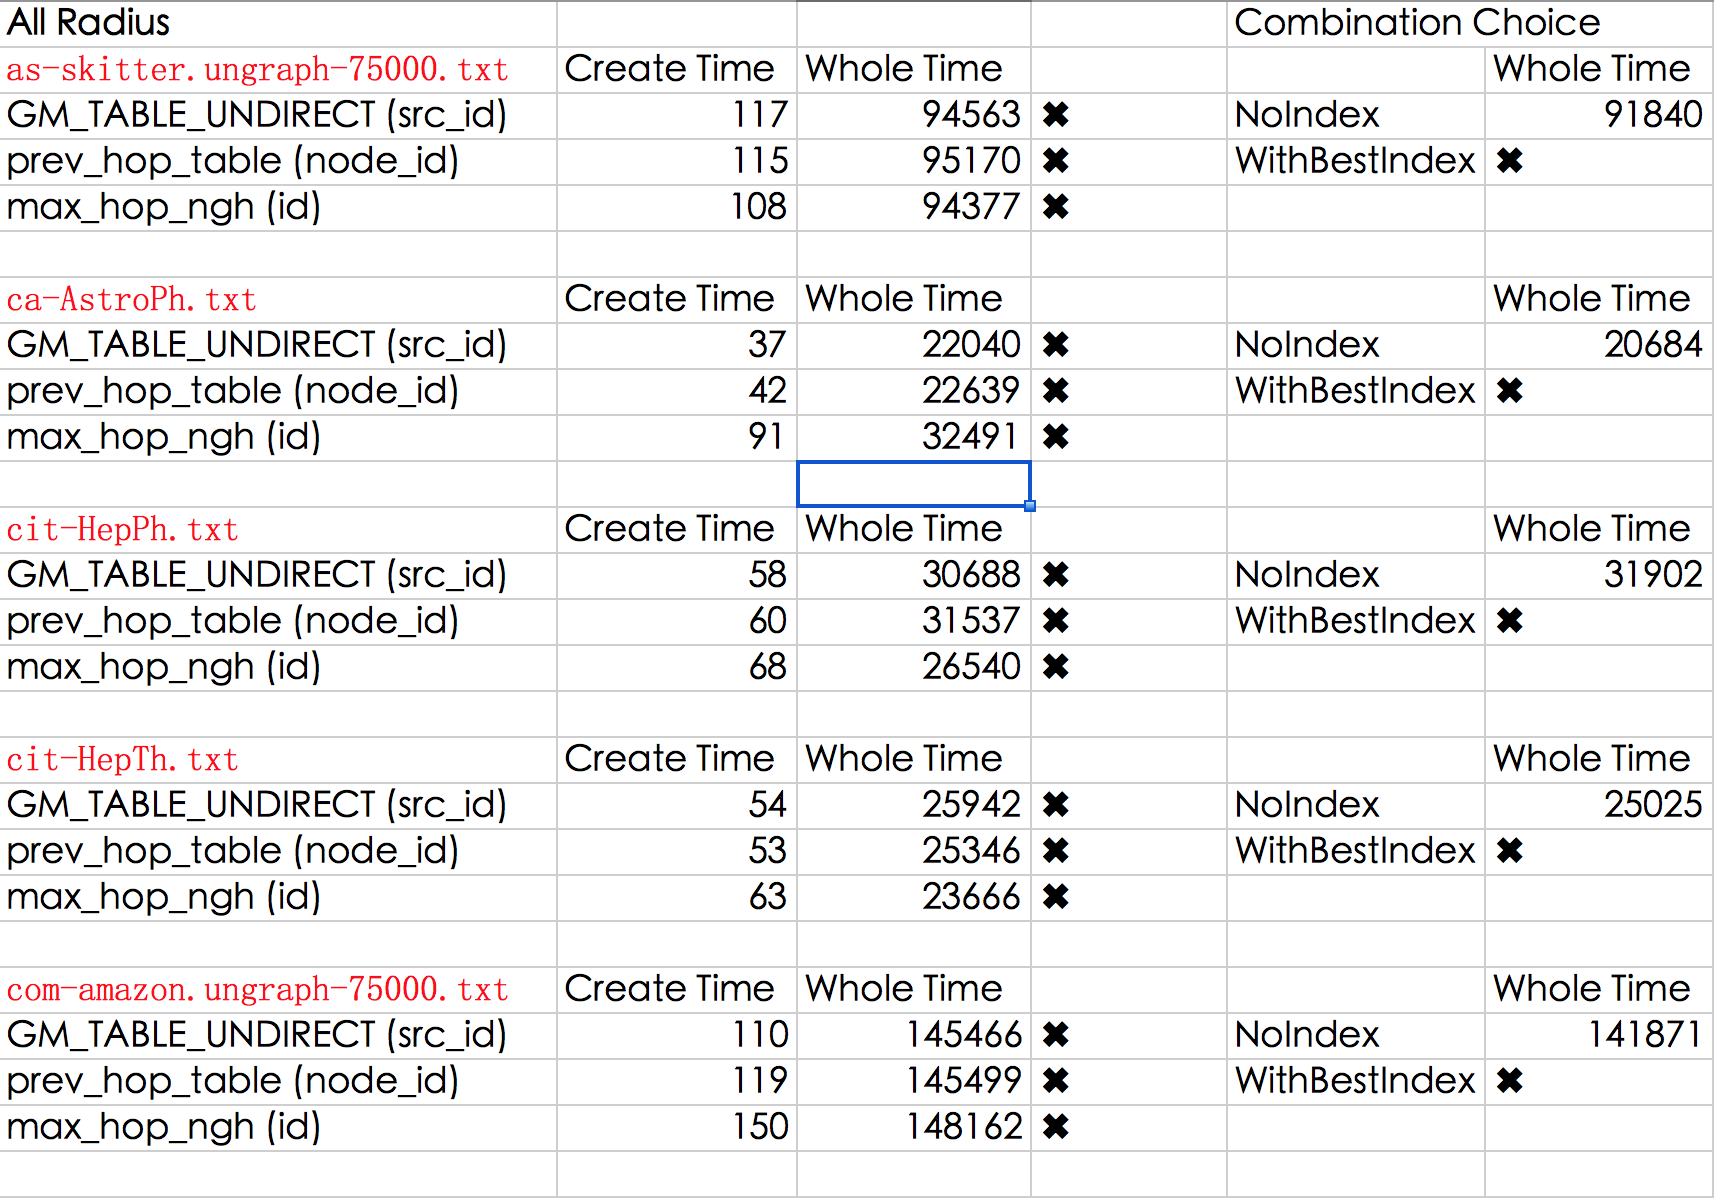
\includegraphics[width=1.0\textwidth]{FIG/AllRadius1.png} \\
     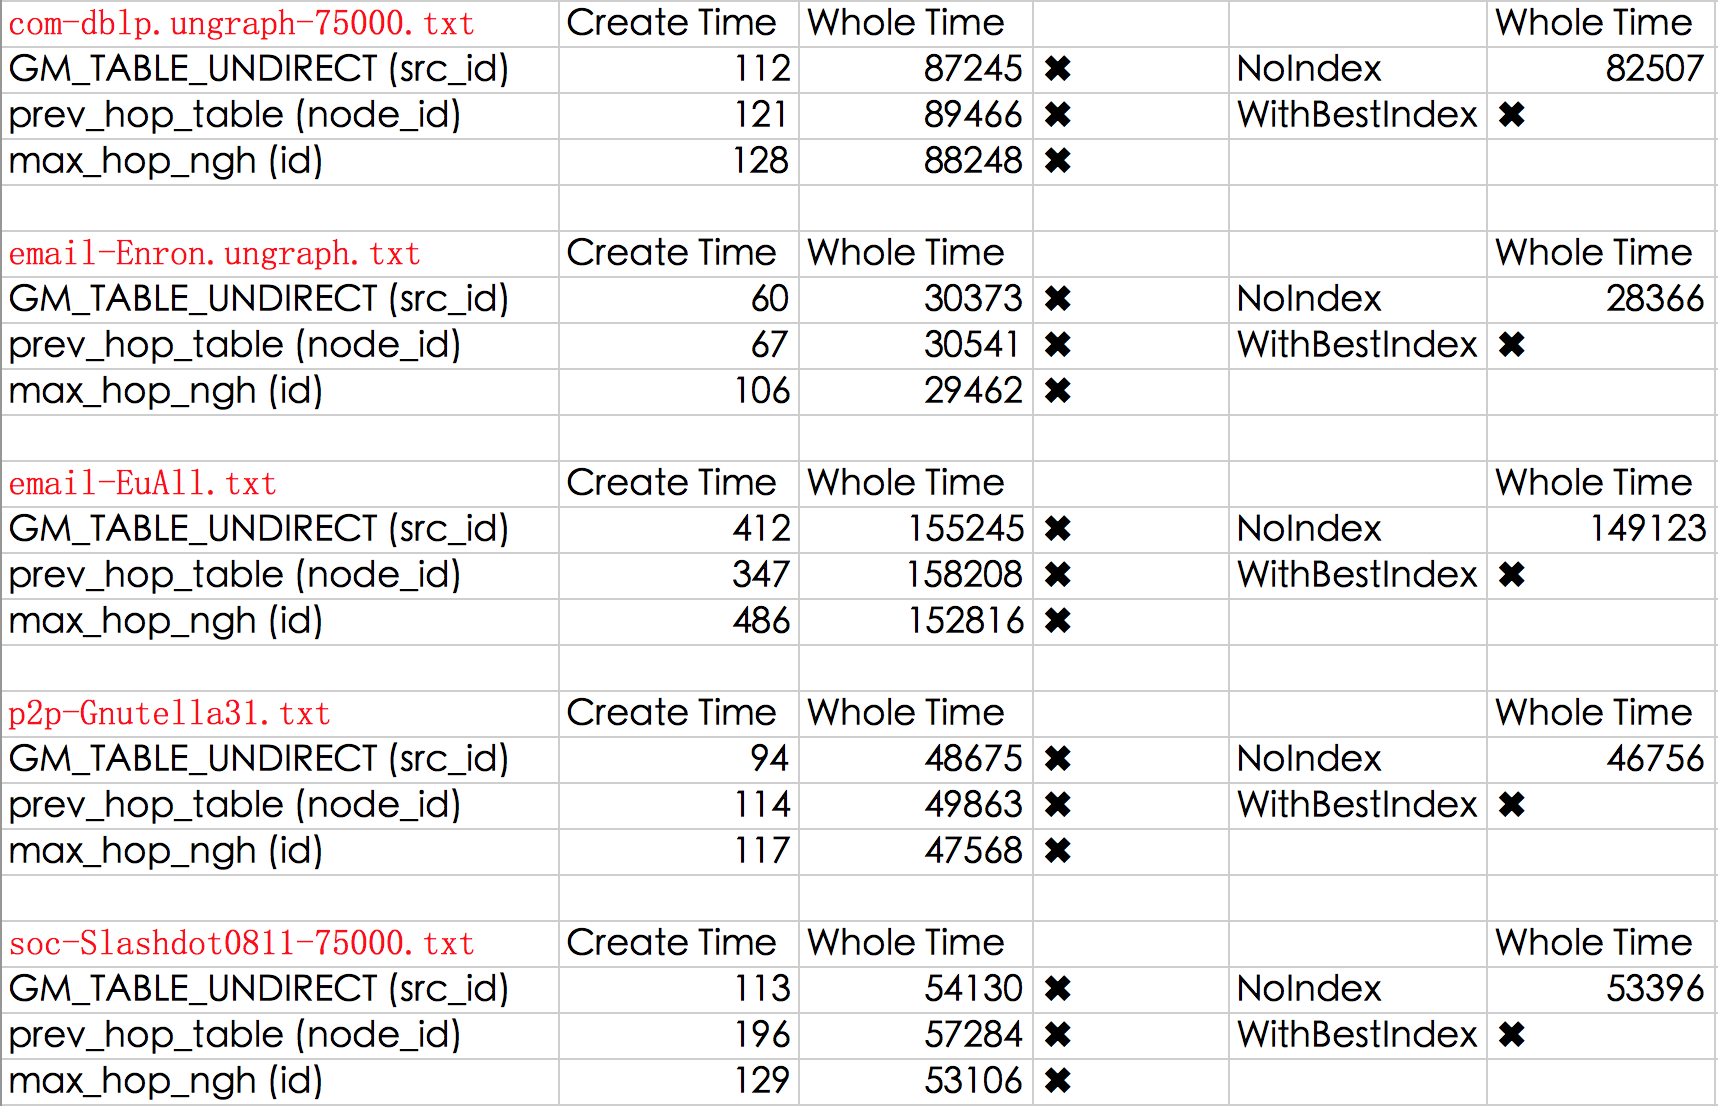
\includegraphics[width=1.0\textwidth]{FIG/AllRadius2.png} \\
\end{tabular}
\caption{Creating Index Experiments on All Radius Algorithm}
\end{center}
\end{figure}

\begin{figure}[H]
\begin{center}
\begin{tabular}{cc}
     % uncomment the next lines, and give the right ps files
     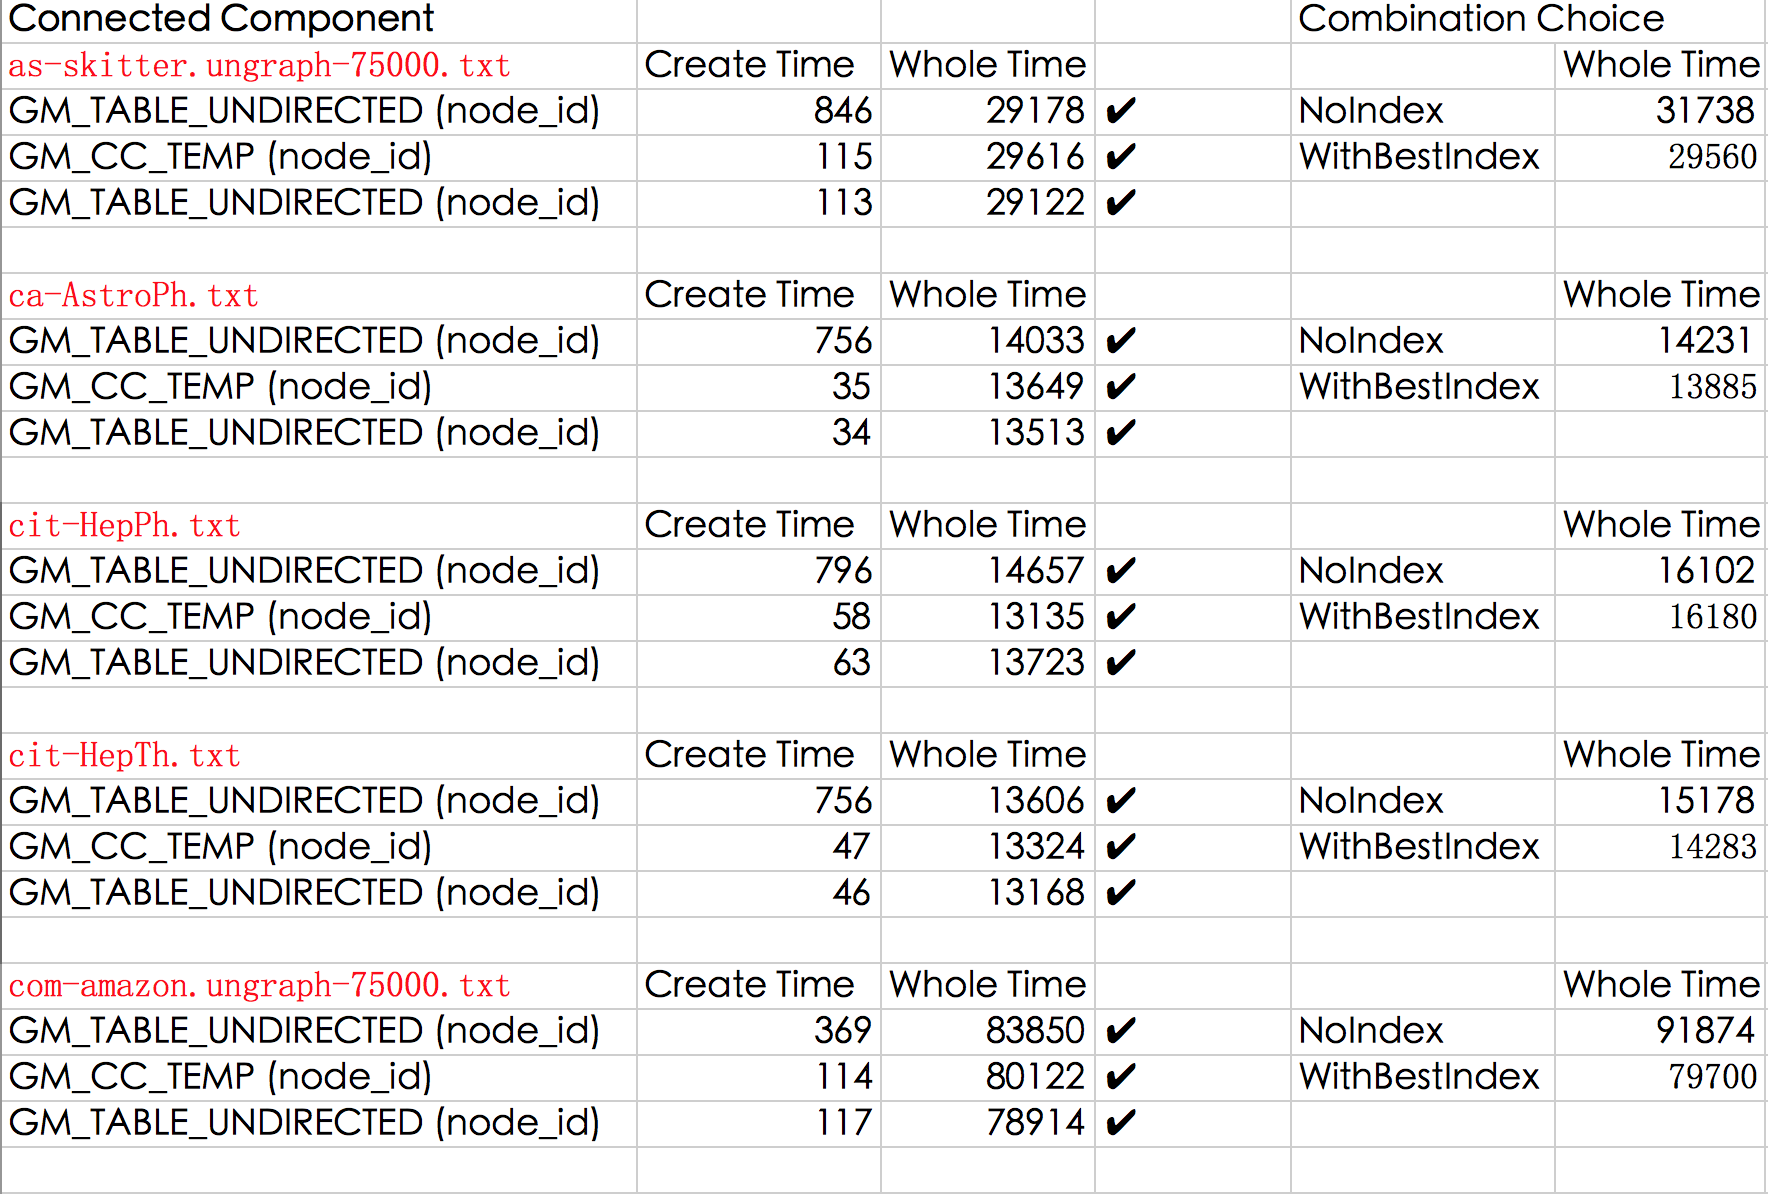
\includegraphics[width=1.0\textwidth]{FIG/CC1.png} \\
     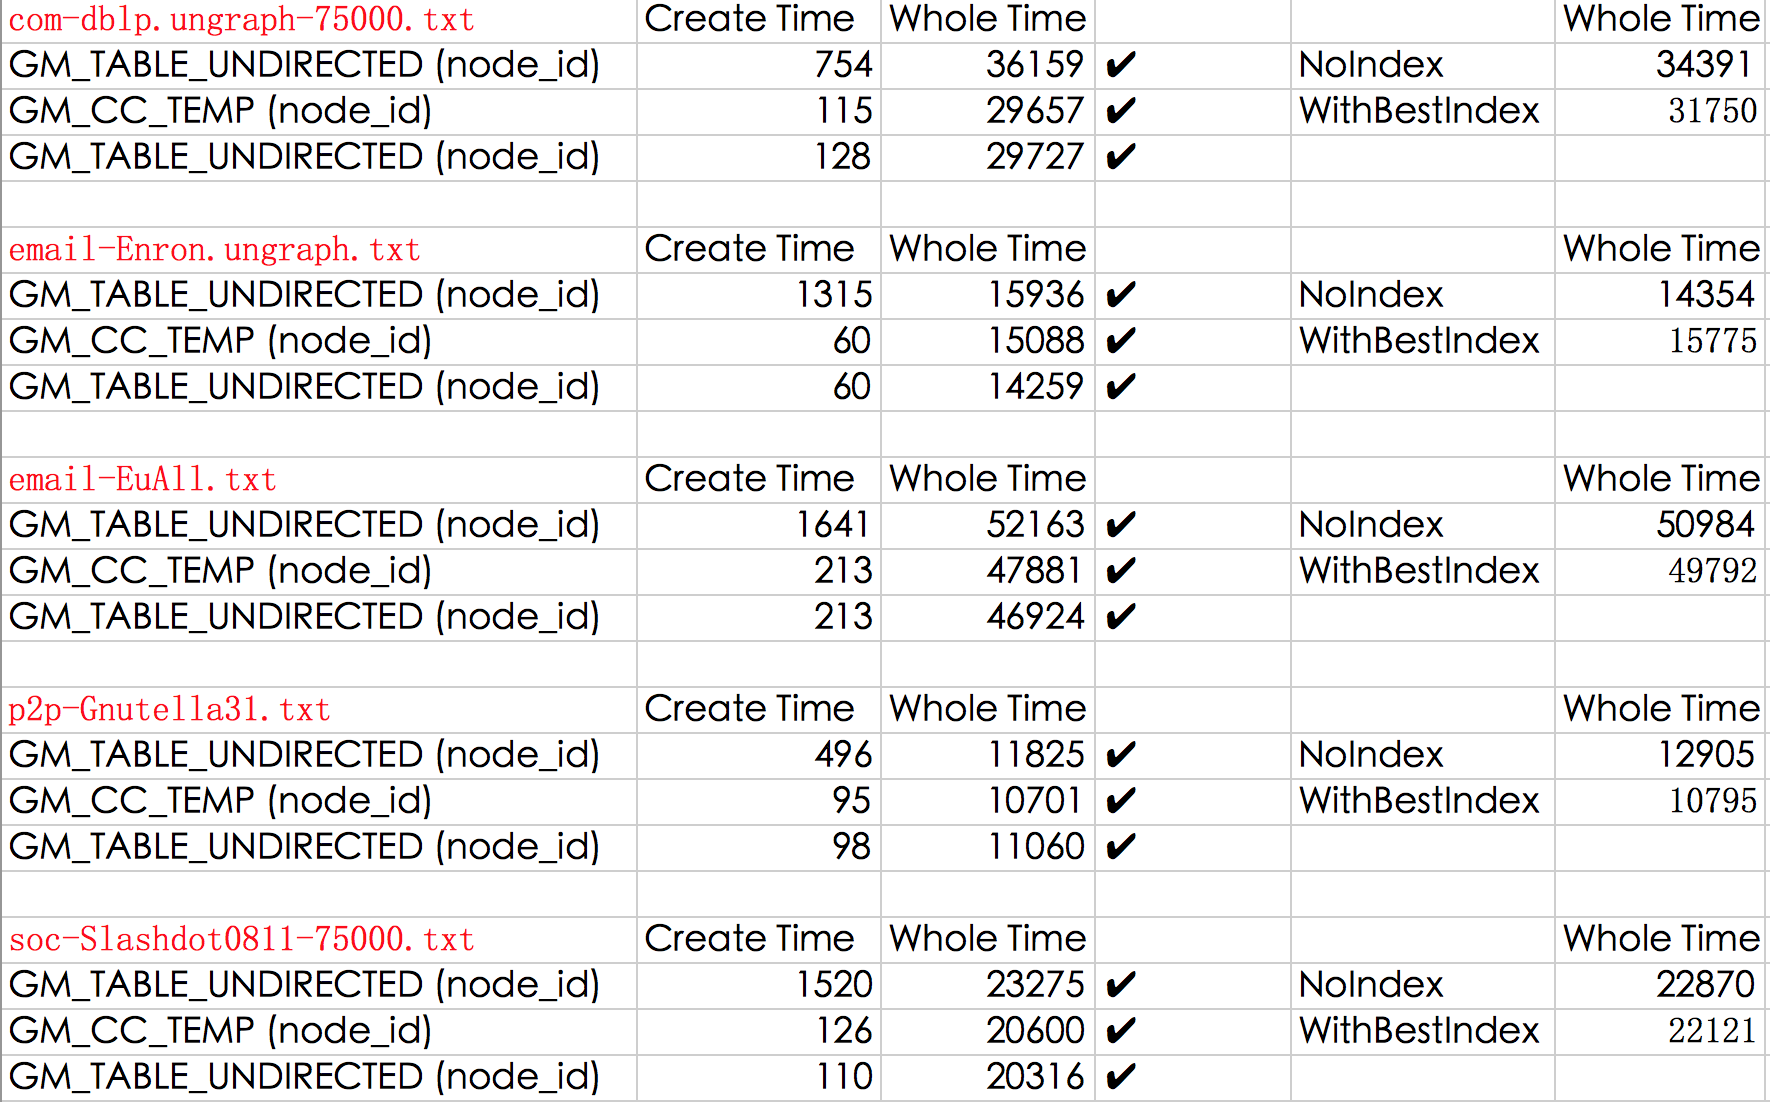
\includegraphics[width=1.0\textwidth]{FIG/CC2.png} \\
\end{tabular}
\caption{Creating Index Experiments on Connected Components Algorithm}
\end{center}
\end{figure}

\begin{figure}[H]
\begin{center}
\begin{tabular}{cc}
     % uncomment the next lines, and give the right ps files
     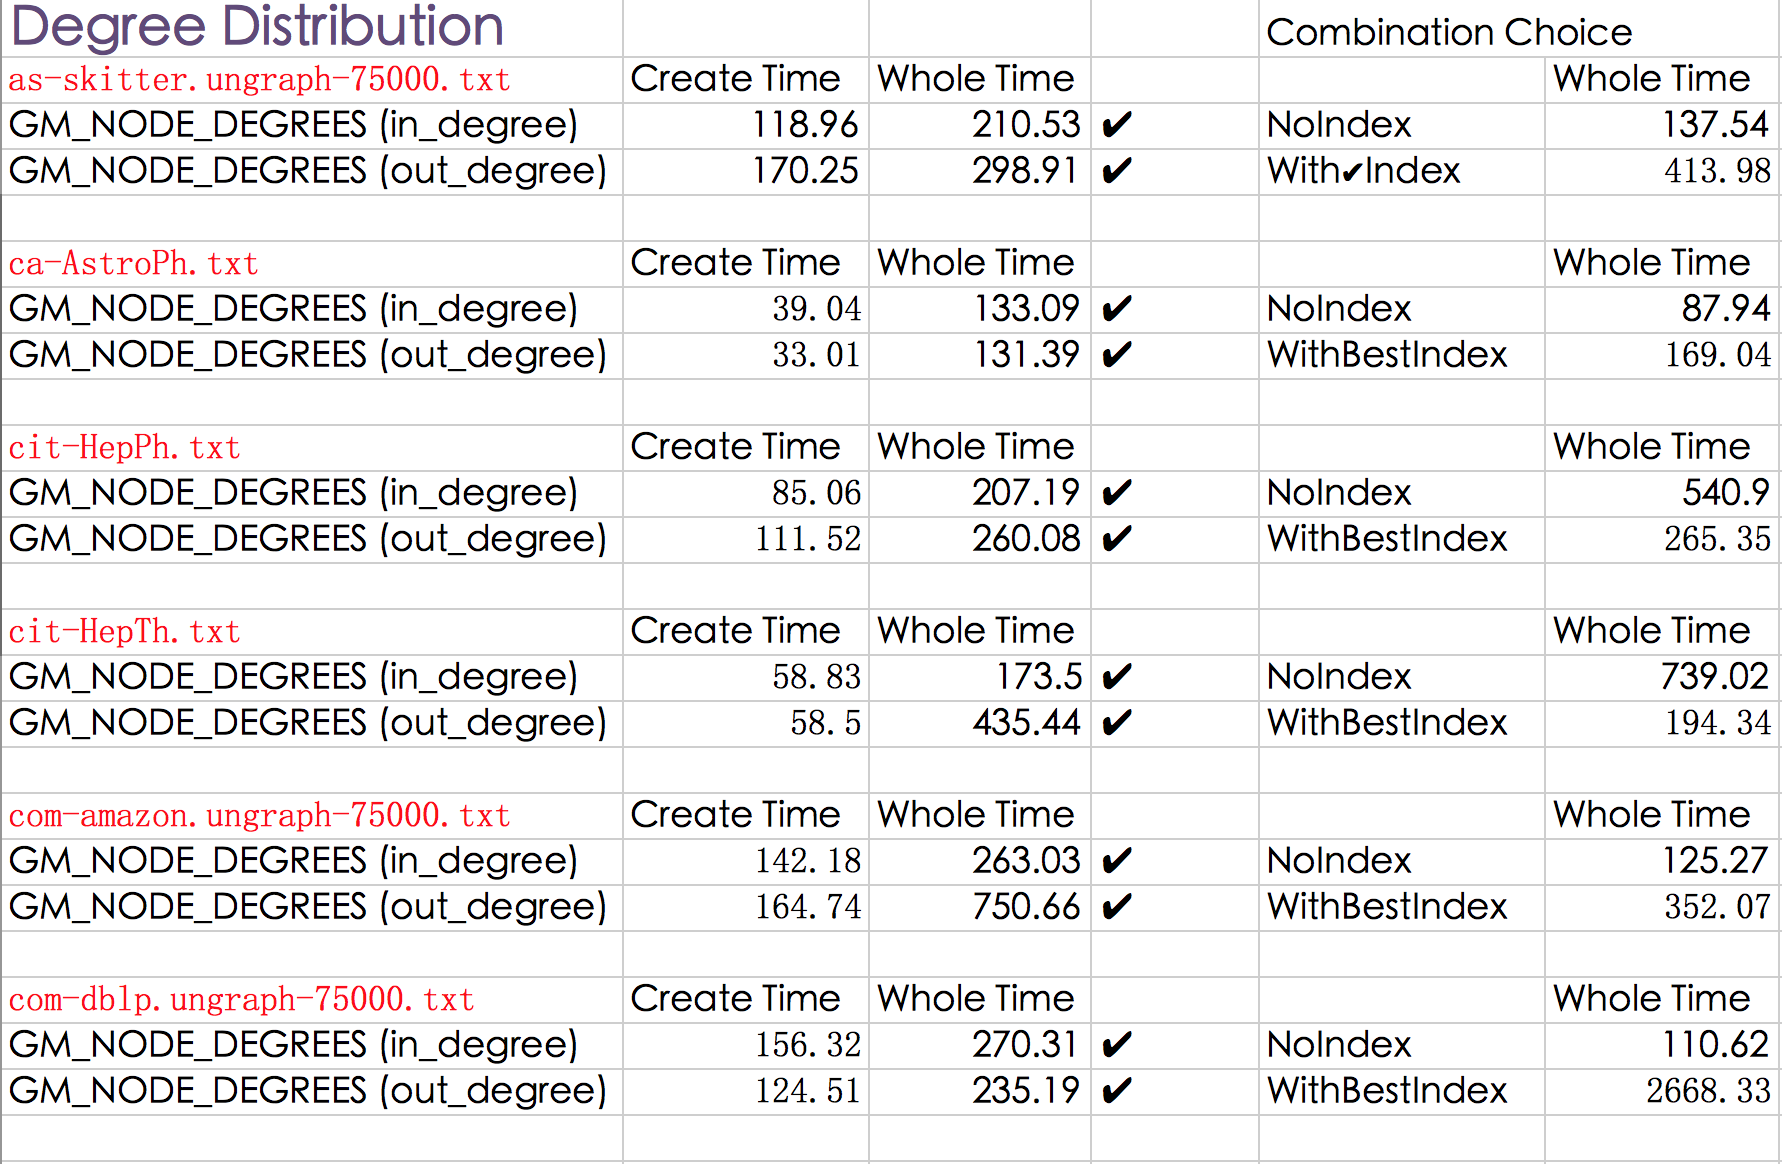
\includegraphics[width=1.0\textwidth]{FIG/DD1.png} \\
     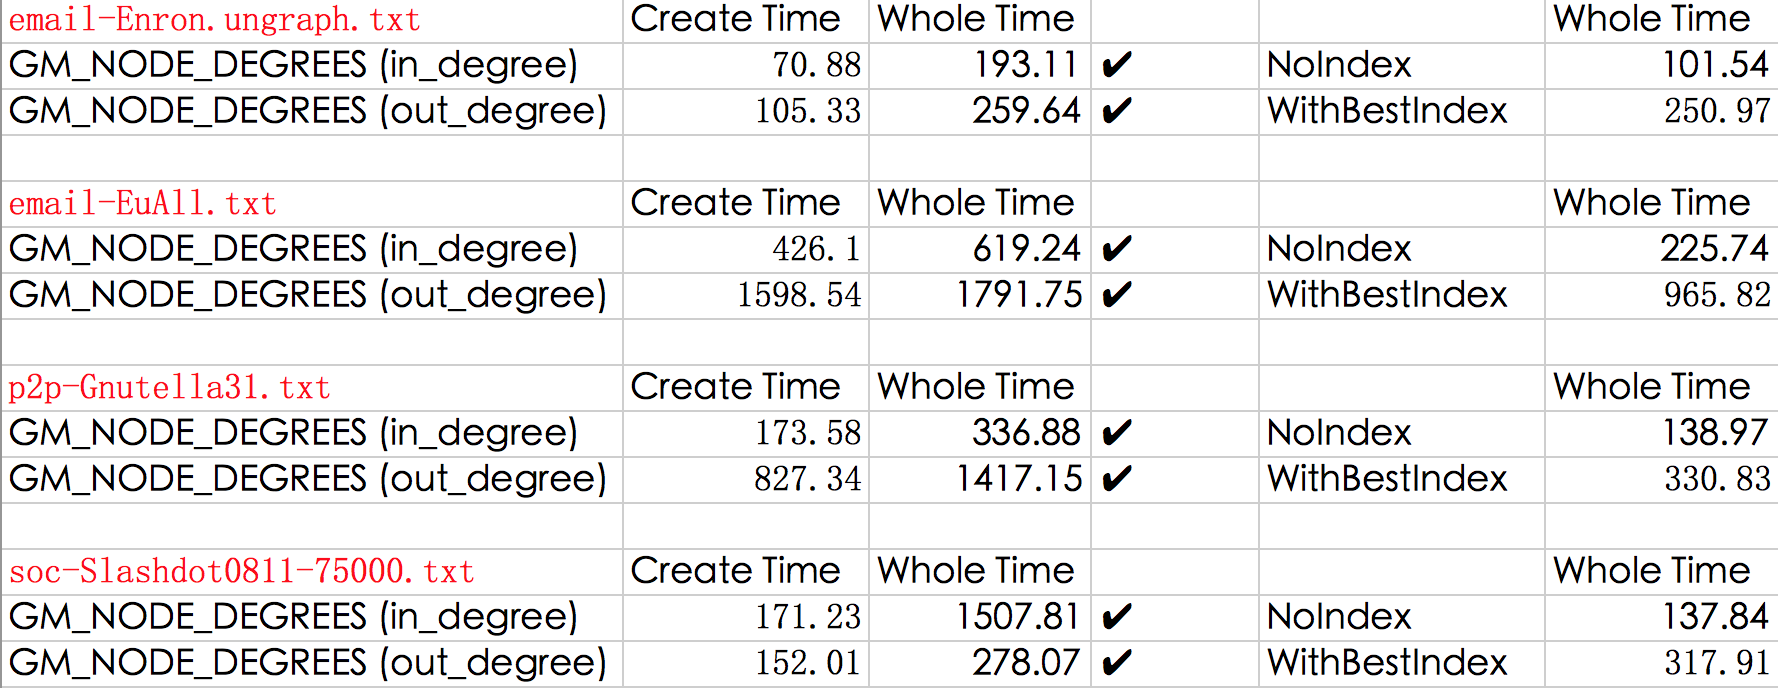
\includegraphics[width=1.0\textwidth]{FIG/DD2.png} \\
\end{tabular}
\caption{Creating Index Experiments on Degree Distribution Algorithm}
\end{center}
\end{figure}

\begin{figure}[H]
\begin{center}
\begin{tabular}{cc}
     % uncomment the next lines, and give the right ps files
     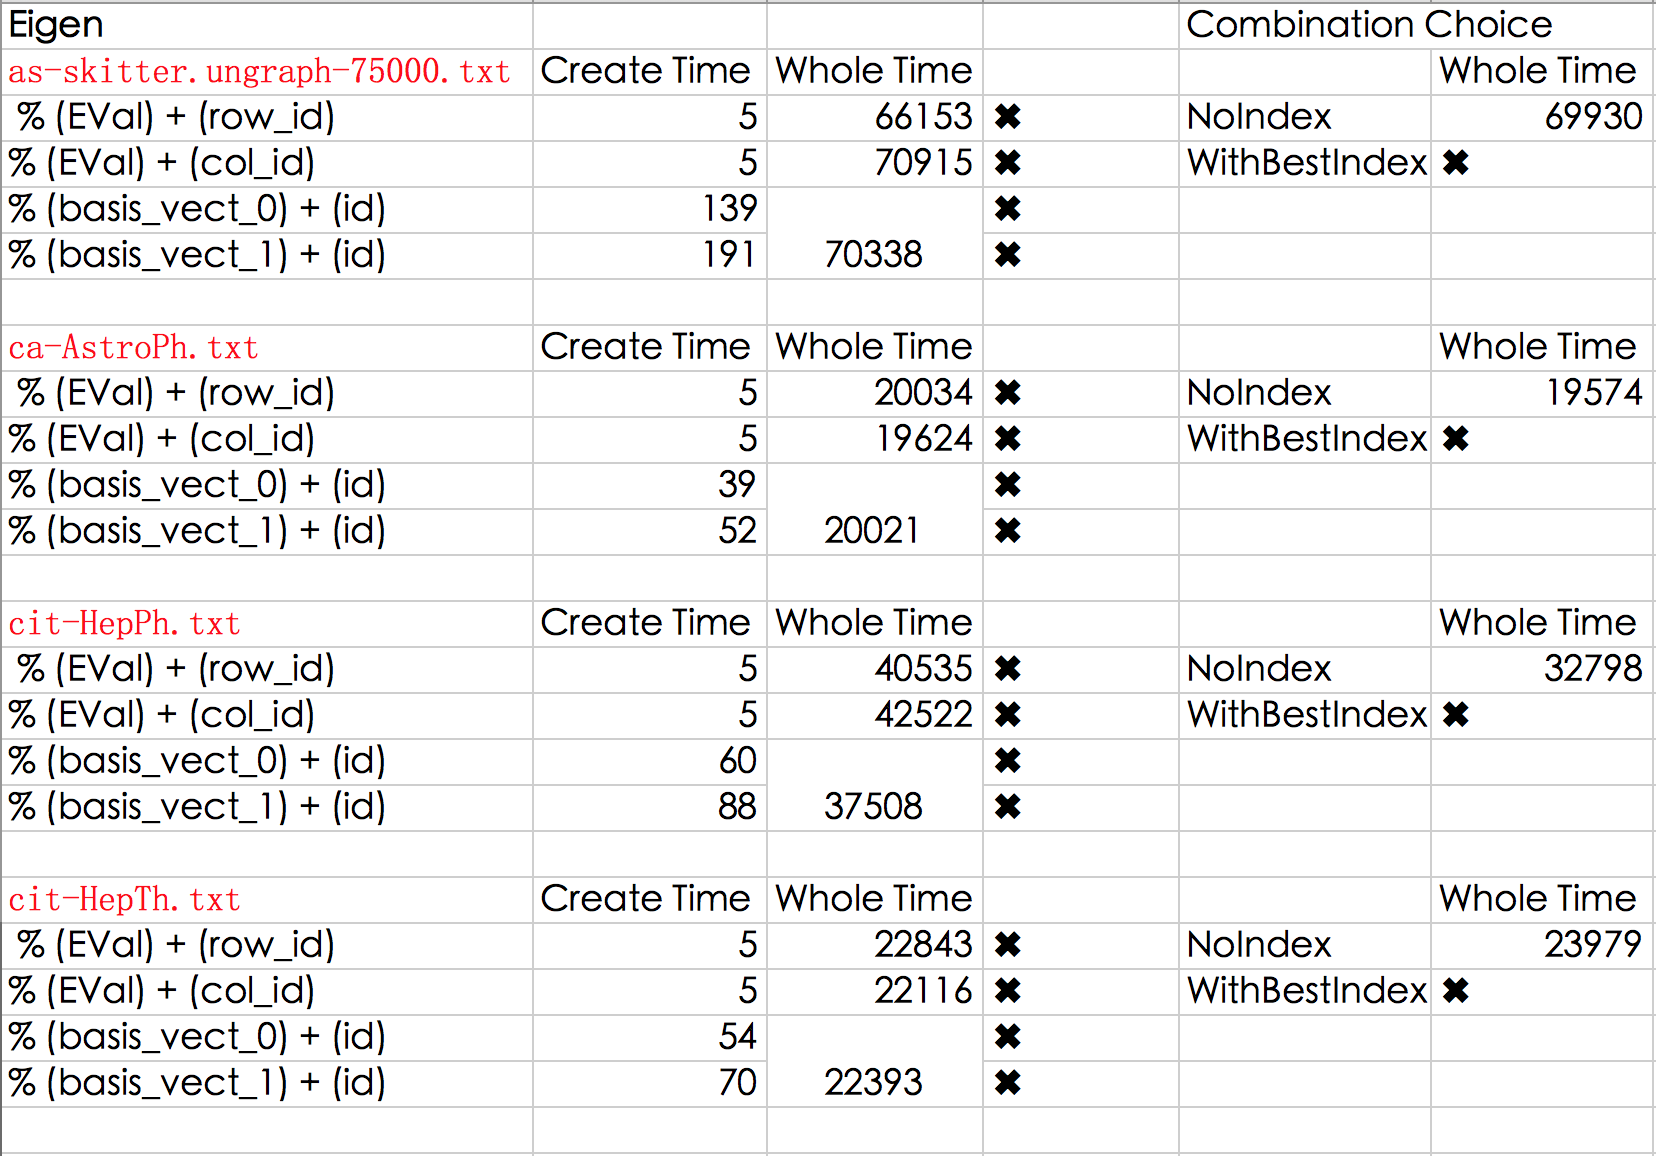
\includegraphics[width=1.0\textwidth]{FIG/Eigen1.png} \\
     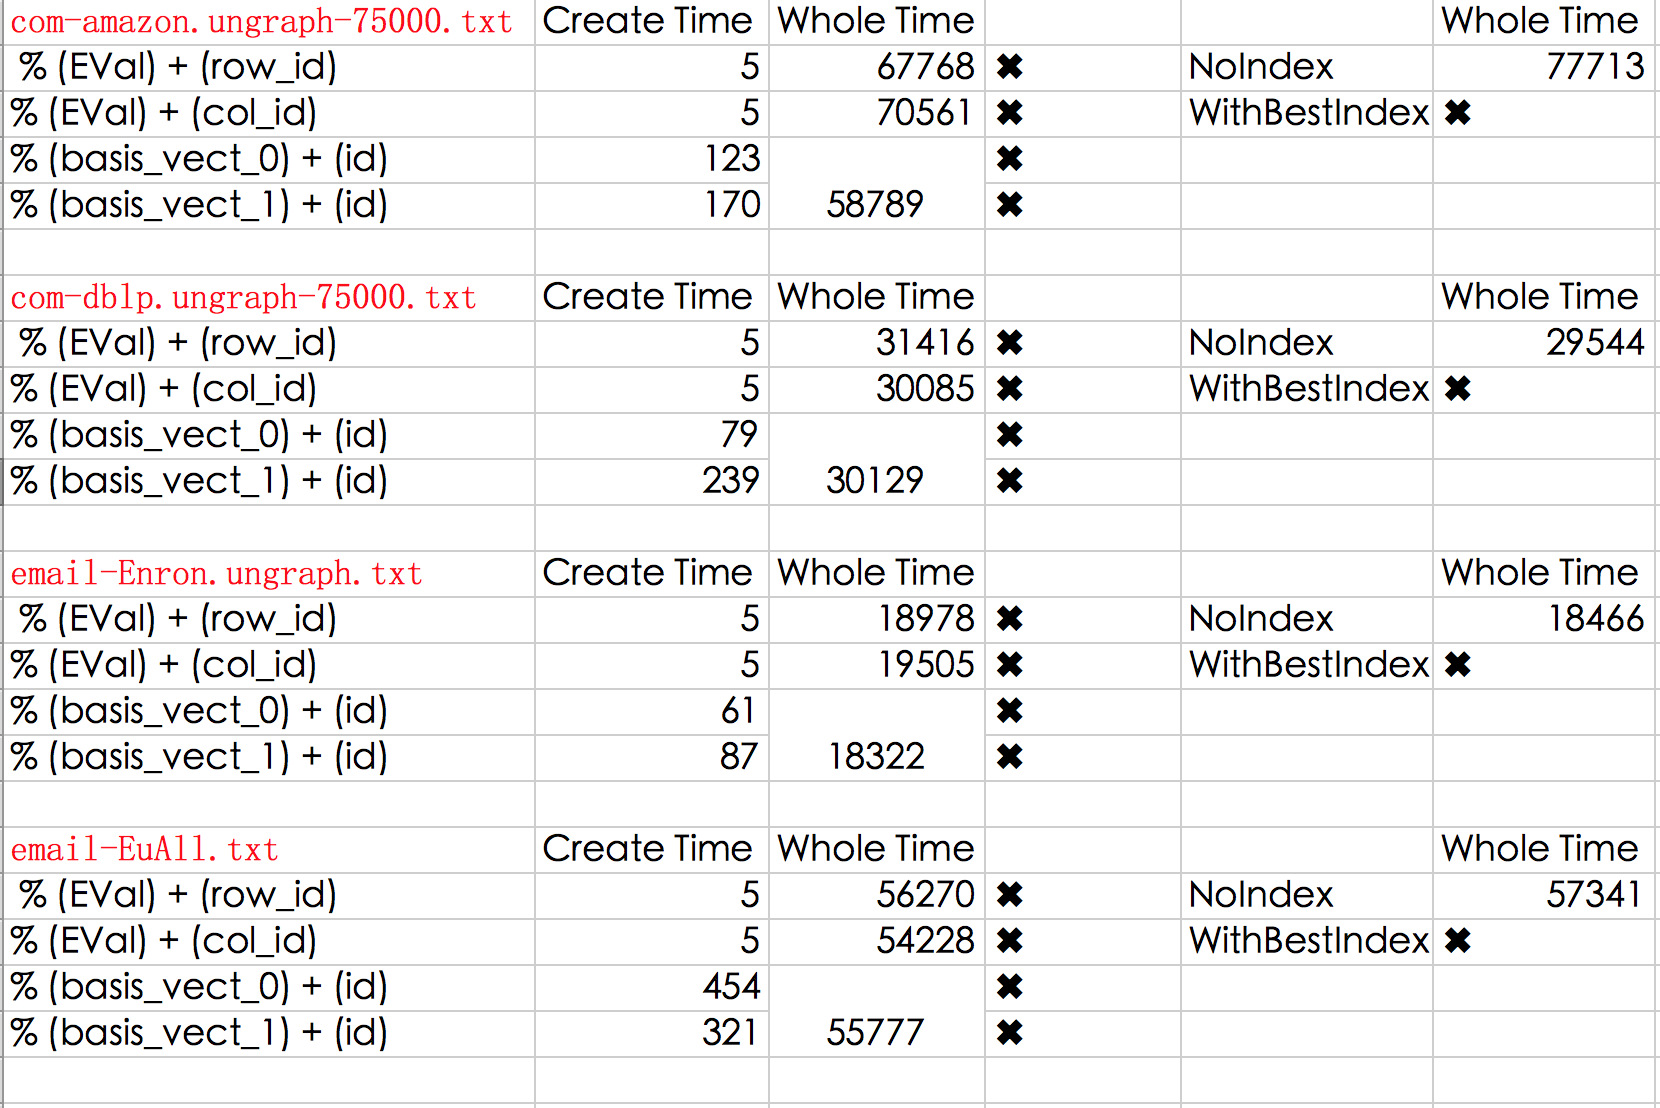
\includegraphics[width=1.0\textwidth]{FIG/Eigen2.png} \\
     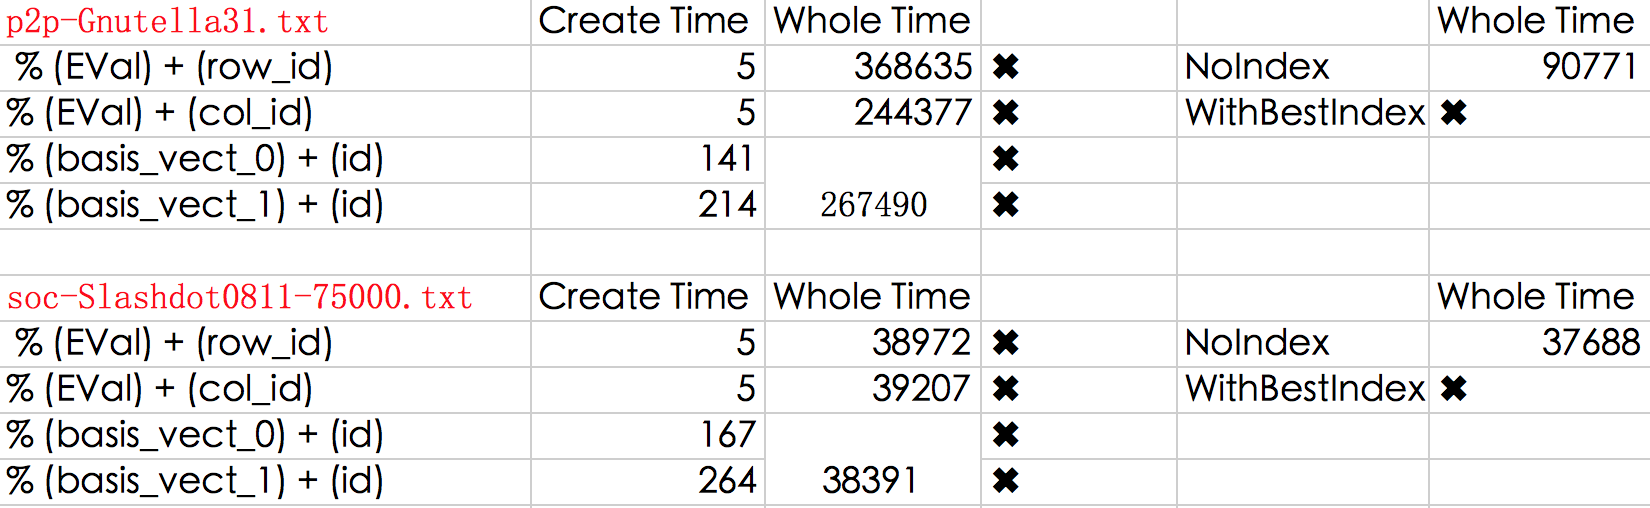
\includegraphics[width=1.0\textwidth]{FIG/Eigen3.png} \\
\end{tabular}
\caption{Creating Index Experiments on Eigen Value Computation Algorithm}
\end{center}
\end{figure}

\begin{figure}[H]
\begin{center}
\begin{tabular}{cc}
     % uncomment the next lines, and give the right ps files
     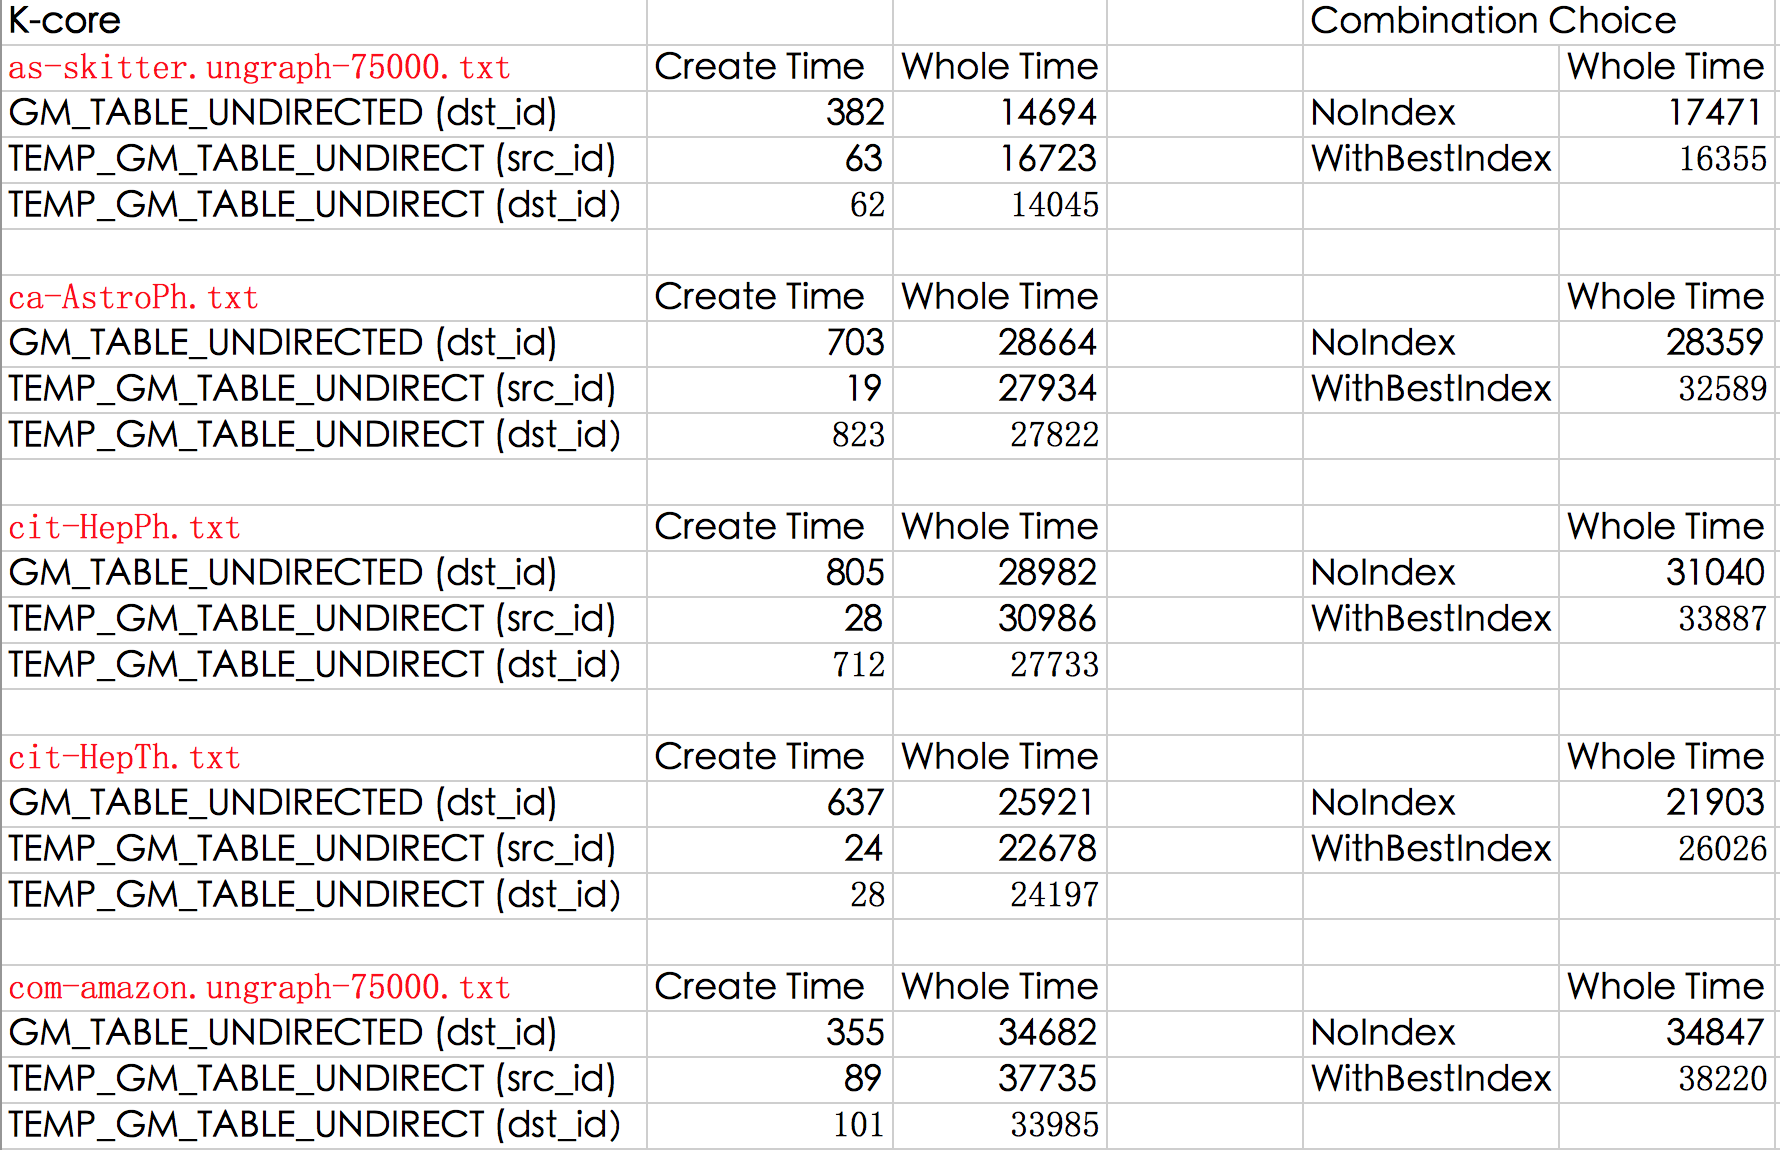
\includegraphics[width=1.0\textwidth]{FIG/KC1.png} \\
     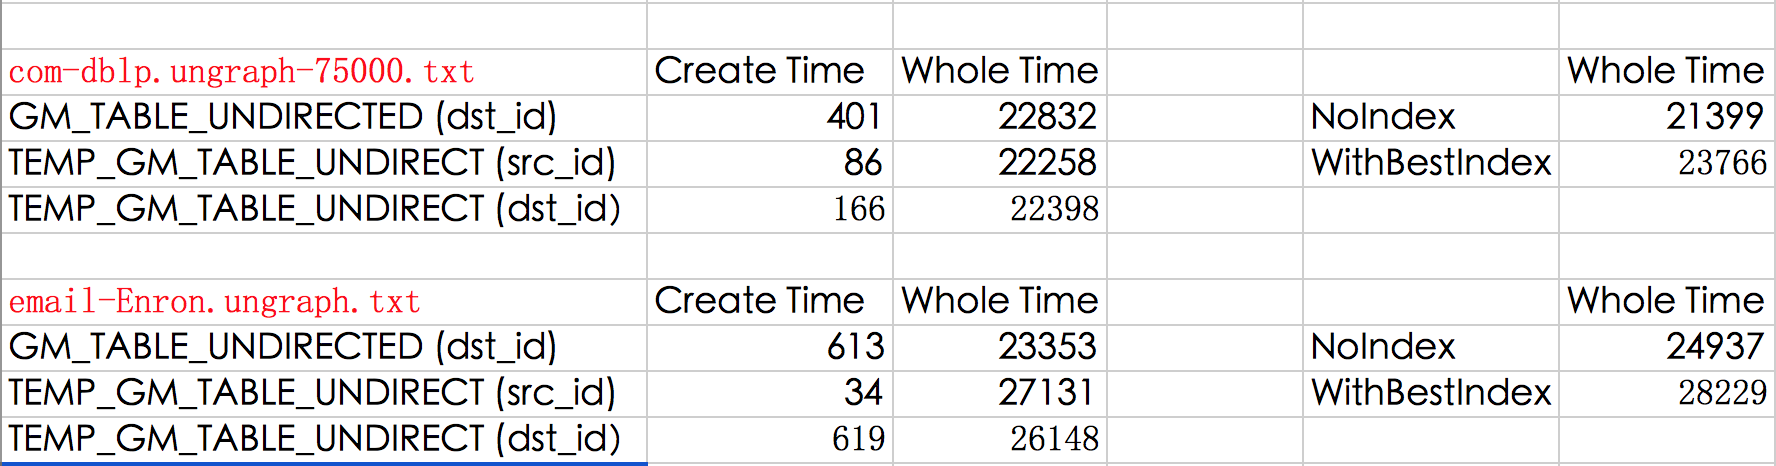
\includegraphics[width=1.0\textwidth]{FIG/KC2.png} \\
\end{tabular}
\caption{Creating Index Experiments on K-core Algorithm}
\end{center}
\end{figure}

\begin{figure}[H]
\begin{center}
\begin{tabular}{cc}
     % uncomment the next lines, and give the right ps files
     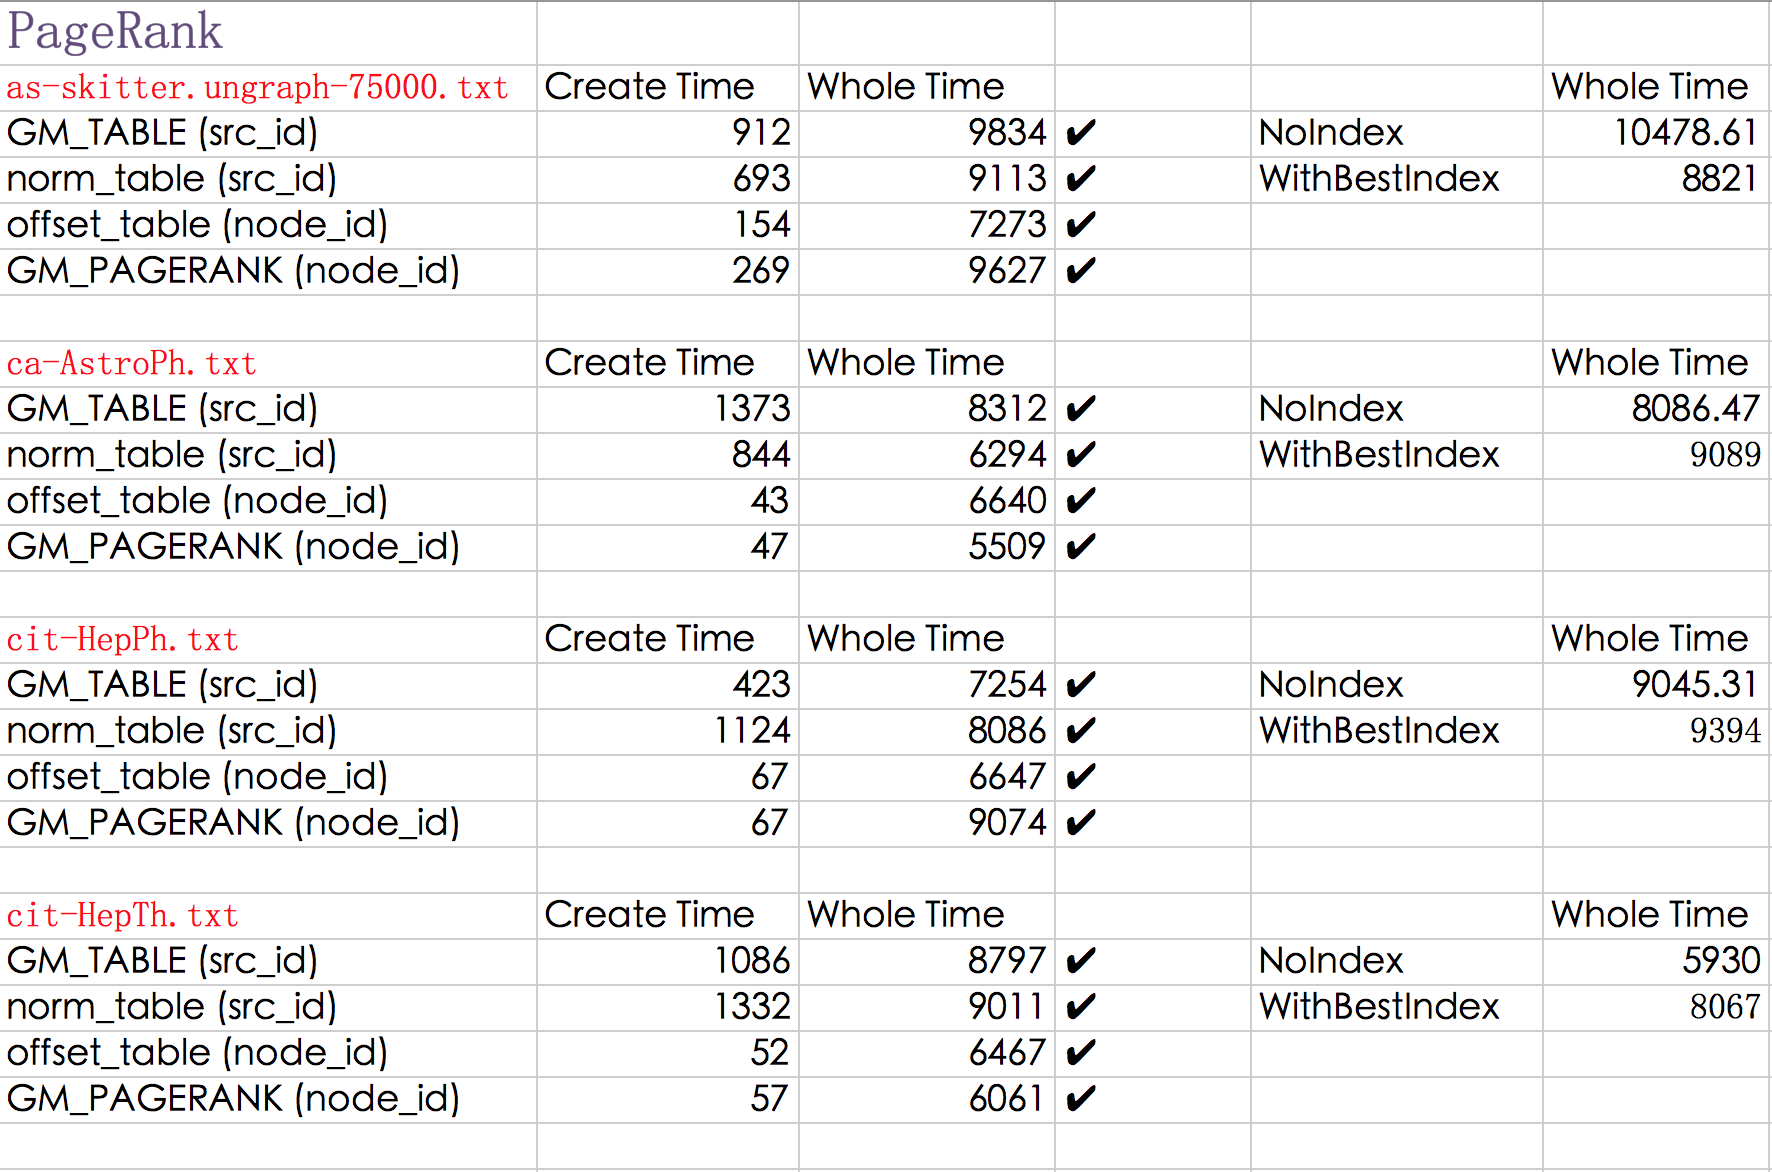
\includegraphics[width=1.0\textwidth]{FIG/PR1.png} \\
     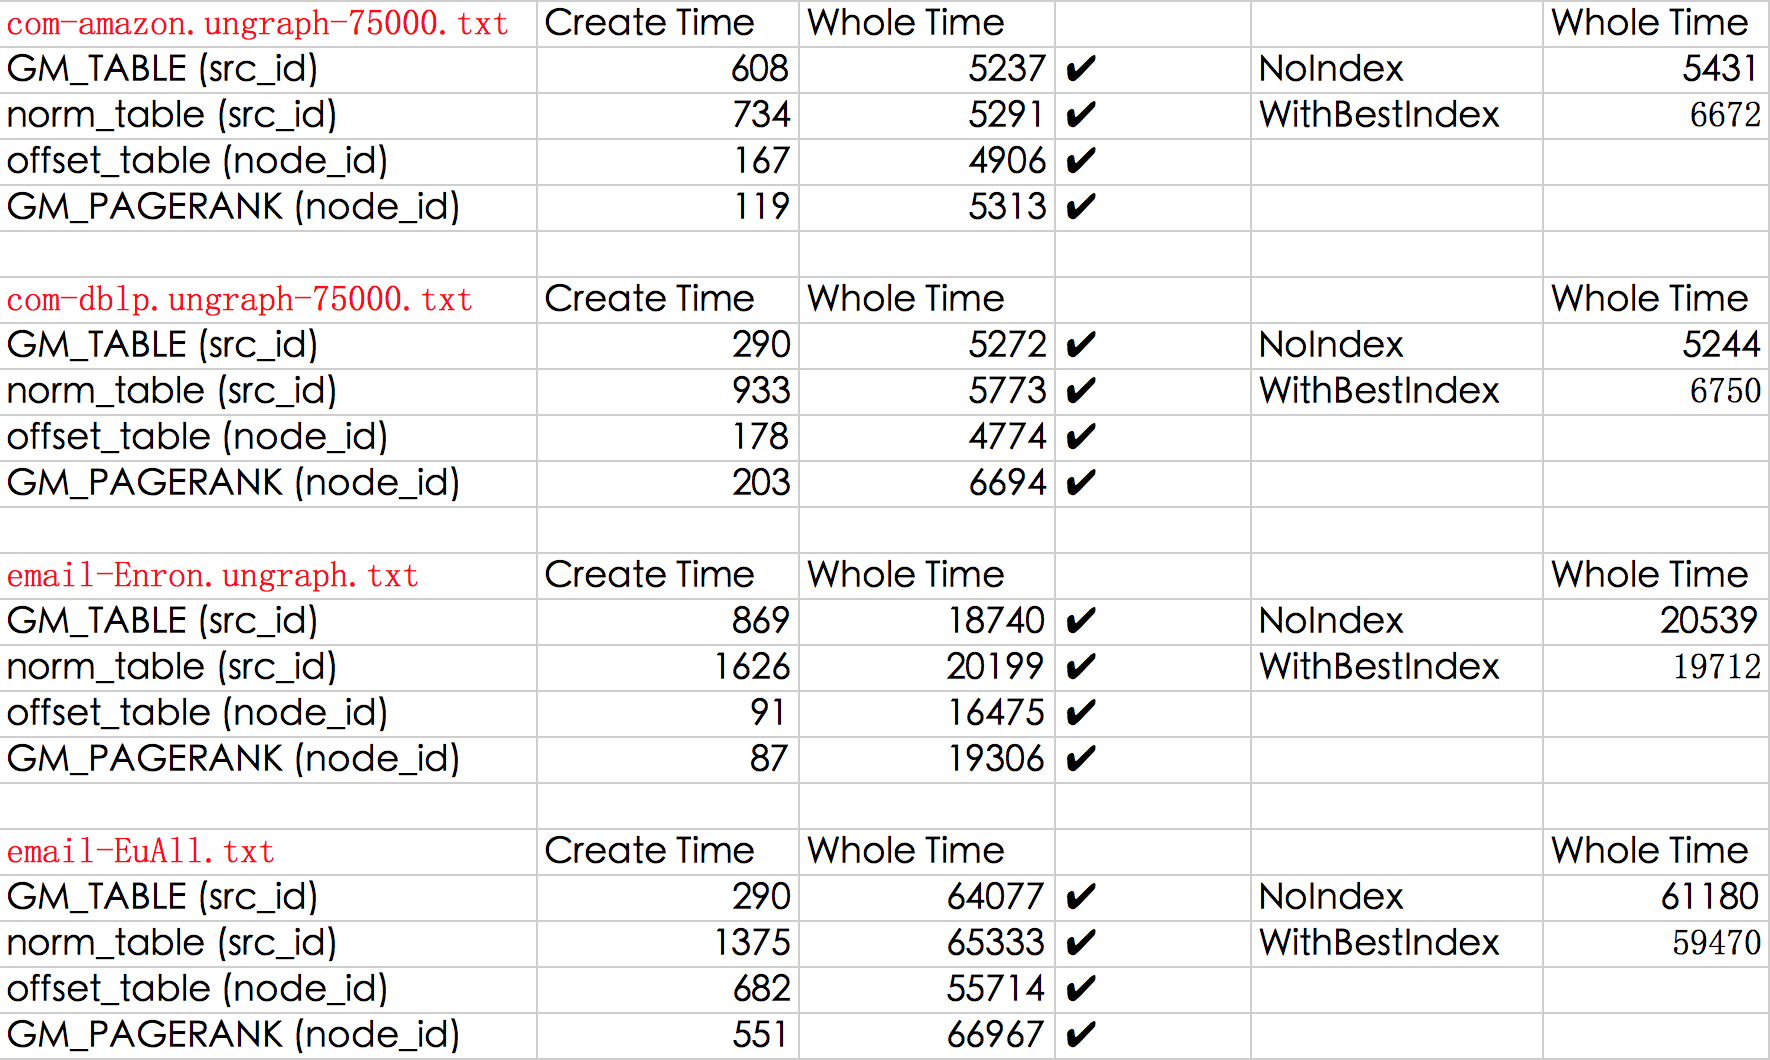
\includegraphics[width=1.0\textwidth]{FIG/PR2.png} \\
\end{tabular}
\caption{Creating Index Experiments on PageRank Algorithm}
\end{center}
\end{figure}


The following are the results of the degree distribution and pagerank results for the ten datasets.
\begin{figure}[H]
\begin{center}
\begin{tabular}{cc}
     % uncomment the next lines, and give the right ps files
     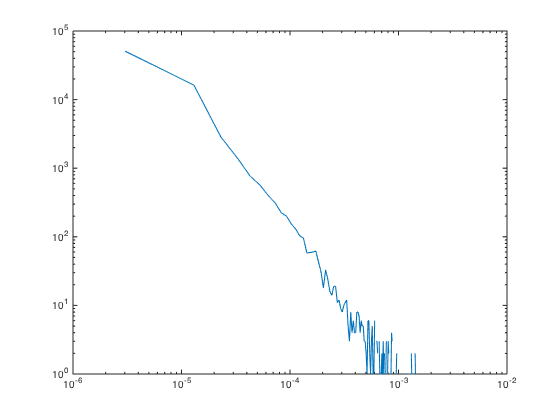
\includegraphics[width=0.3\textwidth]{FIG/1pagerank.png} &
     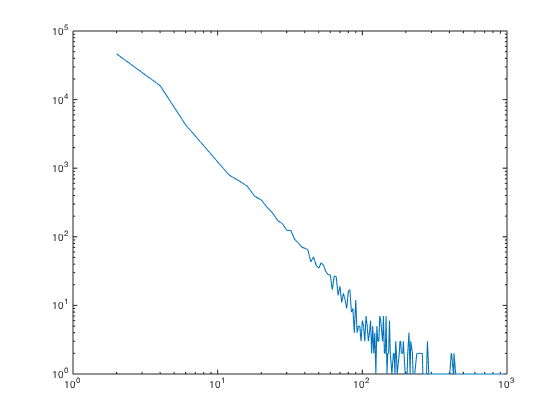
\includegraphics[width=0.3\textwidth]{FIG/1degreedist.png} \\
\end{tabular}
\caption{Result on PageRank Algorithm and Degree Distribution}
\end{center}
\end{figure}

\begin{figure}[H]
\begin{center}
\begin{tabular}{cc}
     % uncomment the next lines, and give the right ps files
     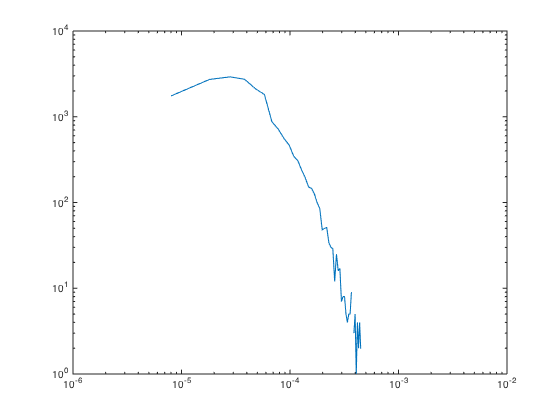
\includegraphics[width=0.3\textwidth]{FIG/2pagerank.png} &
     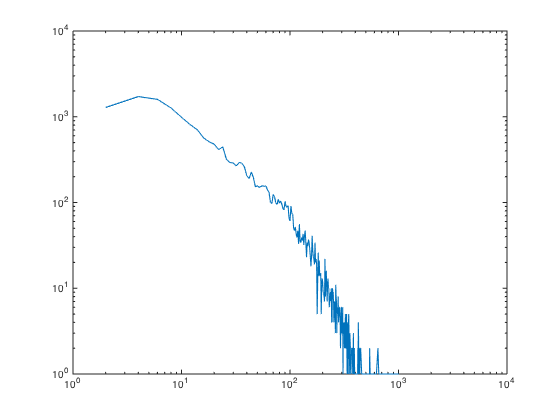
\includegraphics[width=0.3\textwidth]{FIG/2degreedist.png} \\
\end{tabular}
\caption{Result on PageRank Algorithm and Degree Distribution}
\end{center}
\end{figure}

\begin{figure}[H]
\begin{center}
\begin{tabular}{cc}
     % uncomment the next lines, and give the right ps files
     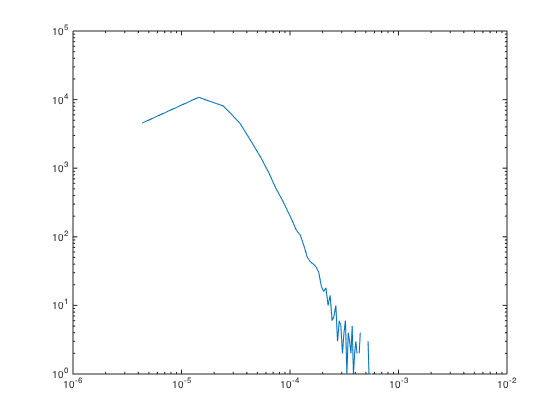
\includegraphics[width=0.3\textwidth]{FIG/3pagerank.png} &
     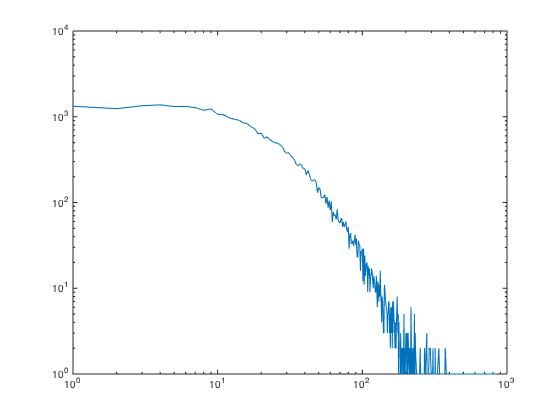
\includegraphics[width=0.3\textwidth]{FIG/3degreedist.png} \\
\end{tabular}
\caption{Result on PageRank Algorithm and Degree Distribution}
\end{center}
\end{figure}

\begin{figure}[H]
\begin{center}
\begin{tabular}{cc}
     % uncomment the next lines, and give the right ps files
     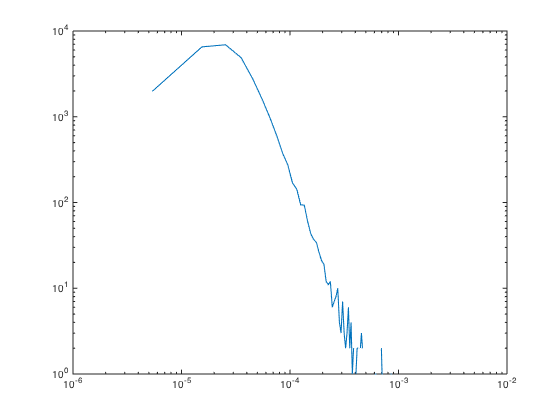
\includegraphics[width=0.3\textwidth]{FIG/4pagerank.png} &
     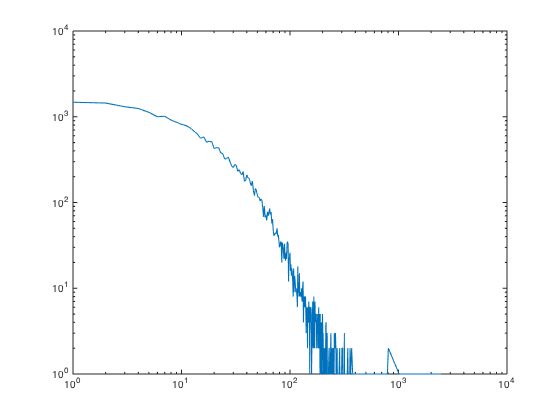
\includegraphics[width=0.3\textwidth]{FIG/4degreedist.png} \\
\end{tabular}
\caption{Result on PageRank Algorithm and Degree Distribution}
\end{center}
\end{figure}

\begin{figure}[H]
\begin{center}
\begin{tabular}{cc}
     % uncomment the next lines, and give the right ps files
     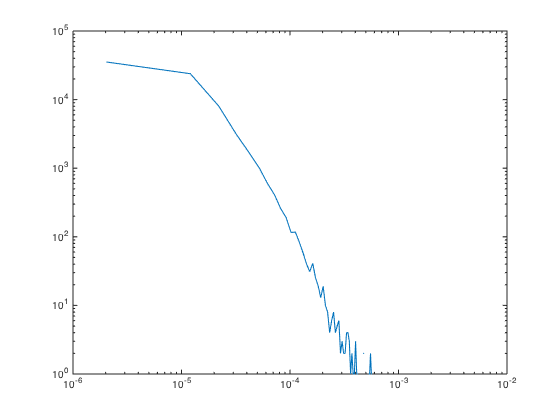
\includegraphics[width=0.3\textwidth]{FIG/5pagerank.png} &
     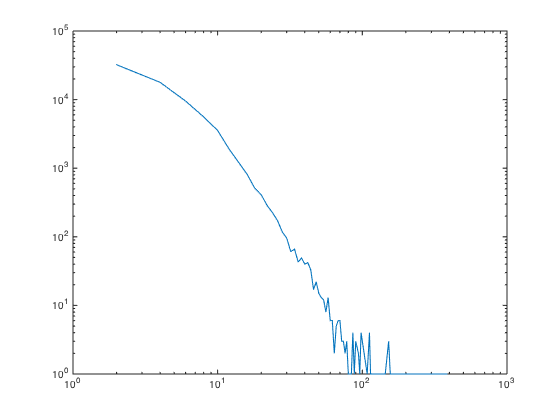
\includegraphics[width=0.3\textwidth]{FIG/5degreedist.png} \\
\end{tabular}
\caption{Result on PageRank Algorithm and Degree Distribution}
\end{center}
\end{figure}

\begin{figure}[H]
\begin{center}
\begin{tabular}{cc}
     % uncomment the next lines, and give the right ps files
     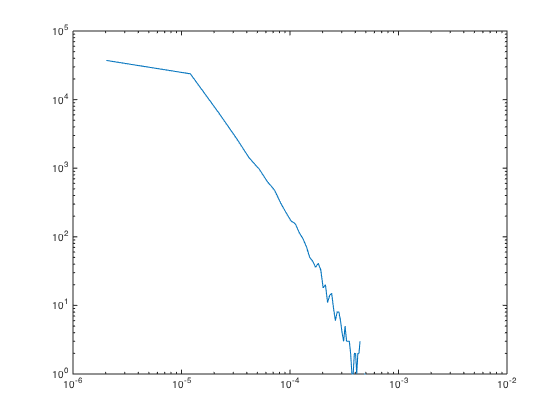
\includegraphics[width=0.3\textwidth]{FIG/6pagerank.png} &
     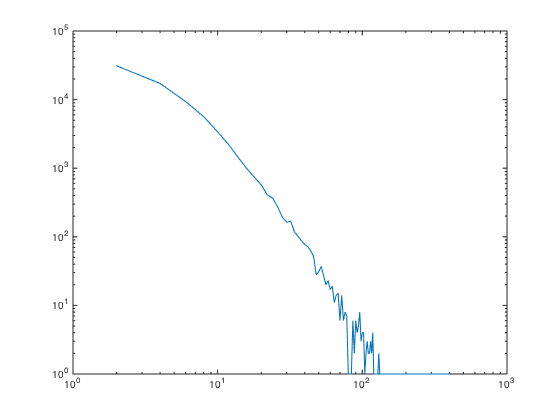
\includegraphics[width=0.3\textwidth]{FIG/6degreedist.png} \\
\end{tabular}
\caption{Result on PageRank Algorithm and Degree Distribution}
\end{center}
\end{figure}

\begin{figure}[H]
\begin{center}
\begin{tabular}{cc}
     % uncomment the next lines, and give the right ps files
     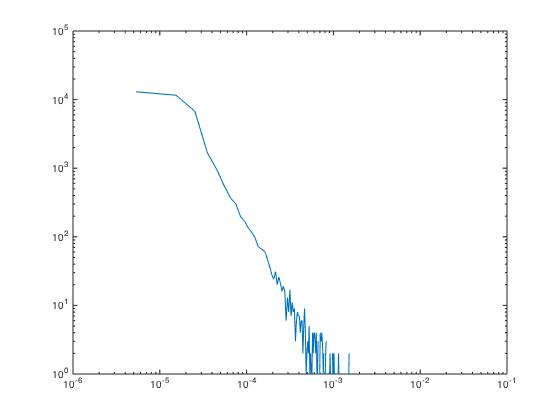
\includegraphics[width=0.3\textwidth]{FIG/7pagerank.png} &
     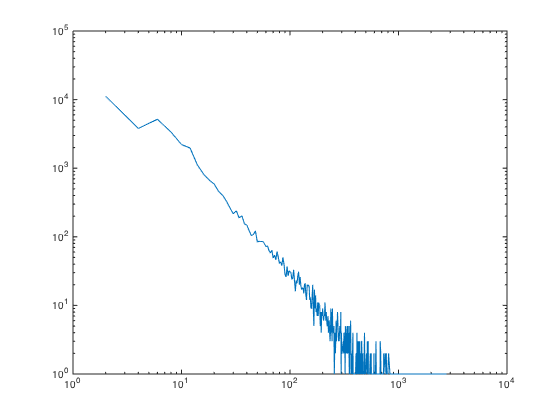
\includegraphics[width=0.3\textwidth]{FIG/7degreedist.png} \\
\end{tabular}
\caption{Result on PageRank Algorithm and Degree Distribution}
\end{center}
\end{figure}

\begin{figure}[H]
\begin{center}
\begin{tabular}{cc}
     % uncomment the next lines, and give the right ps files
     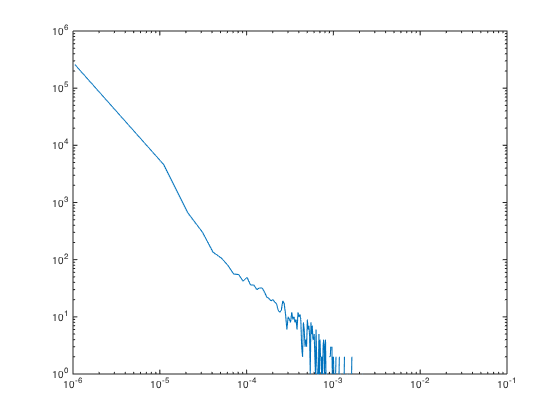
\includegraphics[width=0.3\textwidth]{FIG/8pagerank.png} &
     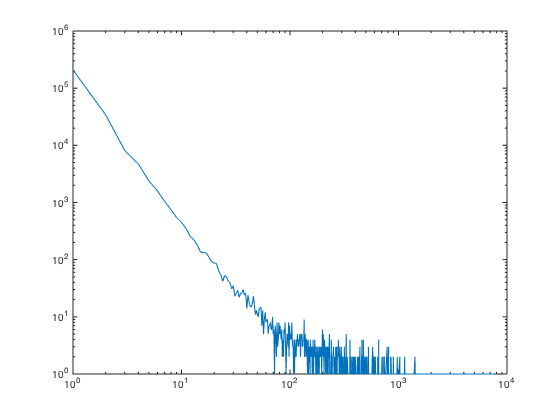
\includegraphics[width=0.3\textwidth]{FIG/8degreedist.png} \\
\end{tabular}
\caption{Result on PageRank Algorithm and Degree Distribution}
\end{center}
\end{figure}

\begin{figure}[H]
\begin{center}
\begin{tabular}{cc}
     % uncomment the next lines, and give the right ps files
     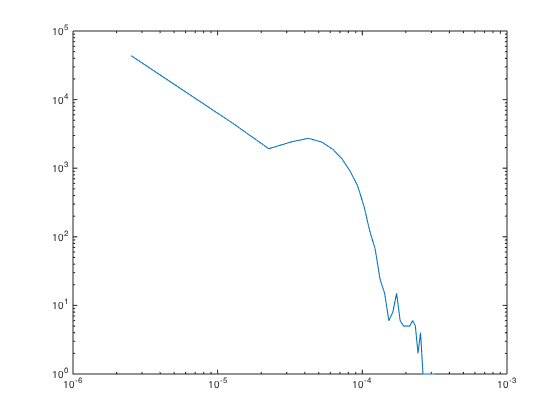
\includegraphics[width=0.3\textwidth]{FIG/9pagerank.png} &
     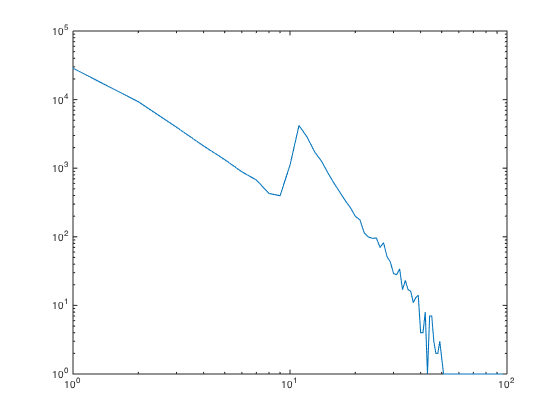
\includegraphics[width=0.3\textwidth]{FIG/9degreedist.png} \\
\end{tabular}
\caption{Result on PageRank Algorithm and Degree Distribution}
\end{center}
\end{figure}

\begin{figure}[H]
\begin{center}
\begin{tabular}{cc}
     % uncomment the next lines, and give the right ps files
     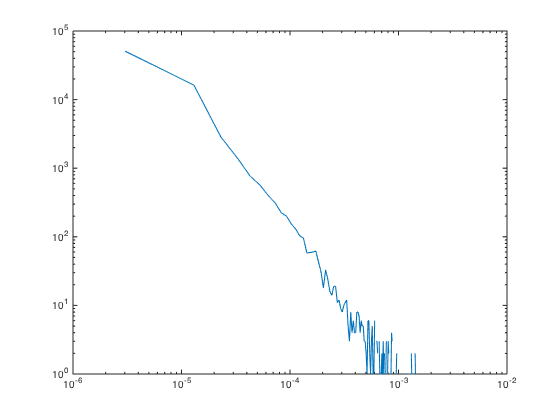
\includegraphics[width=0.3\textwidth]{FIG/1pagerank.png} &
     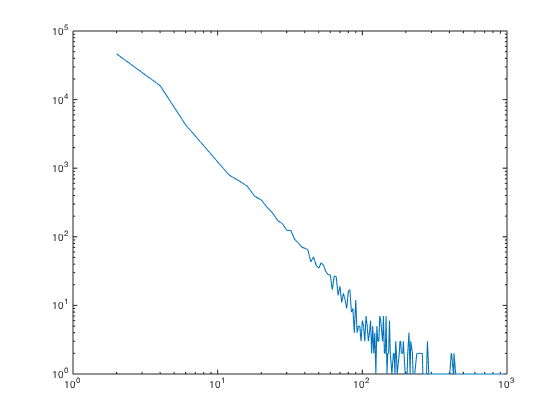
\includegraphics[width=0.3\textwidth]{FIG/1degreedist.png} \\
\end{tabular}
\caption{Result on PageRank Algorithm and Degree Distribution}
\end{center}
\end{figure}

\begin{figure}[H]
\begin{center}
\begin{tabular}{cc}
     % uncomment the next lines, and give the right ps files
     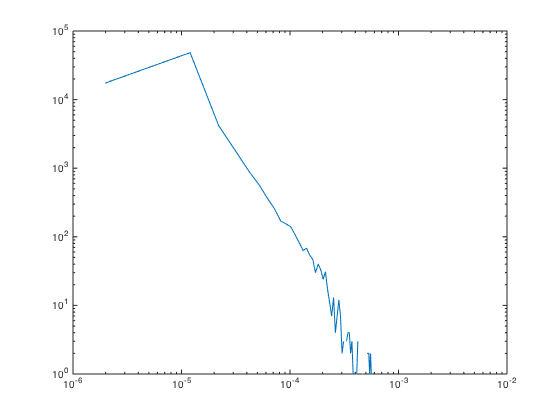
\includegraphics[width=0.3\textwidth]{FIG/10pagerank.png} &
     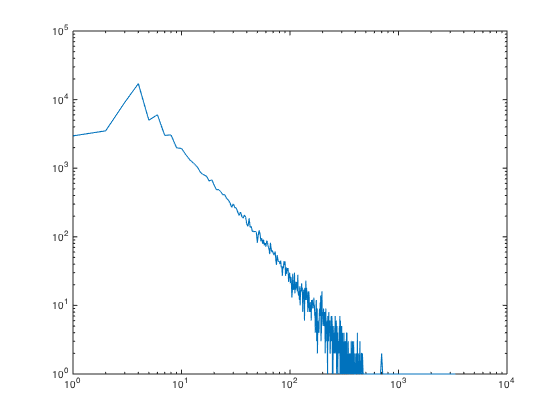
\includegraphics[width=0.3\textwidth]{FIG/10degreedist.png} \\
\end{tabular}
\caption{Result on PageRank Algorithm and Degree Distribution}
\end{center}
\end{figure}


We also did more comprehensive experiments on the 20 datasets to test the functionality of algorithms in the framework and the K-core algorithm we implemented.
Different datasets show different properties when graph mining algorithms are performed on them. We used K = 5 in the experiment as stated in the requirement of the project.

We can find in the table below that some datasets such as \textbf{as-Caida, Cit-HepPh, ca-AstroPh, cit-HepTh, soc-digg, soc-hamsterster, soc-Slashdot0811, text-spanishbook} have relatively big number of nodes but only one or a few connected components. Other datasets such as \textbf{as-skitter, com-amazon, com-dblp, email-Enron} have big number of nodes and relatively big number of connected components. One anomaly type is \textbf{soc-pokec, soc-flickr} in which both number of nodes and number of connected components equal 0. That suggests that no nodes have 5 cores requirement in the dataset. And the small number of connected components suggests that most of the nodes are connected in the graph, only very small number of clusters are formed. The explanation of the formation of connected components is that citations or user relationship form certain groups based on some properties such as interests, regions or languanges.
For example, DBLP dataset has 764 connected components which suggest that many research field are relatively independent and do not cite other areas of research much, resulting in multiple connected components formed. Also, the number of nodes of DBLP is relatively large compared to the original number of nodes, whici is , so we find infer that inside a research area, people cite each other frequently, which helps produce a large number of nodes.
For datasets such as \textbf{soc-hamsterster} and \textbf{cit-HepTh} which include citation information in arXiv's High Energy Physics area and friendships between users of the website hamsterster.com, we can find that only one connected components are formed. The reason is that this is a small area of research or common interest and people in this group are well connected and no significant sub-clusters are formed. The large number of nodes compared to the total number of nodes suggest that research work and users in these fields are highly connected and active, or many of the nodes are of high quality.

For datasets such as \textbf{soc-pokec, soc-flickr} and \textbf{p2p-Gnutella} which no or very few connected components are formed and that the number of nodes in the K-core results are small. The explanation for few connected components are similar to the above, which means that relations of points in the dataset are already highly connected and form a group that no further significant sub-clusters form. The small number of nodes means that nodes such as users in digg.com and flickr.com do not have authorities or hubs who have a lot of followers. Instead, users have simple relationship with each other and are generally equal. Then K=5 K-core algorithm will generate very small number of nodes who have the coreness.

\begin{center}
Table of K-core Algorithm Result for 20 Datasets
\begin{tabular}{ |c|c|c| }
 \hline
 Dataset & Number of Nodes & Number of Connected Components \\
  as-Caida & 1436 & 1 \\
  as-skitter & 9090 & 159 \\
  bio-protein & 57 & 1 \\
  ca-AstroPh & 12574 & 8 \\
  cit-Cora & 384 & 13 \\
  cit-HepPh & 8393 & 3 \\
  cit-HepTh & 21768 & 2 \\
  com-amazon & 19029 & 2090 \\
  com-dblp & 23194 & 764 \\
  email-Enron & 21577 & 180 \\
  p2p-Gnutella31 & 88 & 7 \\
  soc-digg & 1066 & 2 \\
  soc-flickr & 0 & 0 \\
  soc-hamsterster & 1103 & 1 \\
  soc-pokec & 0 & 0 \\
  soc-Slashdot0811 & 20577 & 2 \\
  soc-Youtube & 277 & 4 \\
  soft-jdkdependency & 84 & 1 \\
  text-spanishbook & 1350 & 1 \\
 \hline
\end{tabular}
\end{center}


Eigenvalues Experiment

We performed eigenvalue calculation on the adjacency matrix of undirected graphs as directed graphs' adjacency matrix is not symmetric and eigenvalues of such graphs can be complex numbers. Eigenvalue analysis is fundamental in terms of the spectral properties of graphs. It can also be used to find approximations to graph measures such as triangle counts.  The algorithms implemented in the {\em graphMiner} framework that we used to do the experiments are Lanczos-SO and QR algorithms.

We plotted comparisons of eigen vectors for certain two of top three eigenvalues. Some datasets such as \textbf{soc-Youtube, Euall} show clear "spoke" like features. Datasets such as \textbf{Gnutella31, bio-protein} have no clear "spoke" features. In fact, if we only plot the very top nodes with the largest eigenvalues, the plots will show clearer spokes, for example, if we use top 100 nodes in the datasets with largest eigenvalues. The plots we have used are called EE-plots, showing the values of nodes in the $i_th$ eigenvector vs. in the $j_th$ eigenvector. Notice the clear ‘spokes’ in top eigenvectors signify the existence of a strongly related group of nodes in near-cliques or bi-cliques




\section{Conclusions}
    \label{sec:conclusions}
    The proposed method {\em someMETHOD}
has the following advantages:
\bit
\item it gives better classification accuracy than all 10 competitors we tried
\item its accuracy is very close to the very best competitor
      in the {\em UCR Insect Classification Contest}.
\item it is scalable
\eit



\bibliography{BIB/christosref,BIB/other}
\bibliographystyle{plain}

\newpage
\appendix
\section{Appendix}

\subsection{Labor Division}

The team performed the following tasks
\bit
\item Implementation of Kcore [Jin Hu]
\item Unit Tests and visualization of results [Ye Zhou]
\item General debugging and testing[Ye Zhou and Jin Hu]
\eit

\subsection{Code for K-core}

\begin{lstlisting}

import argparse

from gm_params import *
from gm_sql import *
from math import sqrt
import os
import time

db_conn = None;


# Convert directed to undirected + remove multiple edges
def gm_to_undirected(rm_multiple = True):
    cur = db_conn.cursor()
    gm_sql_table_drop_create(db_conn, GM_TABLE_UNDIRECT, "src_id integer, dst_id integer, weight real")

    if rm_multiple:
        stmt = "INSERT INTO %s " % (GM_TABLE_UNDIRECT) + \
                    " SELECT src_id, dst_id, AVG(weight) FROM " + \
                    " (SELECT src_id, dst_id, weight FROM %s " % (GM_TABLE) + \
                    " UNION ALL" + \
                    " SELECT dst_id \"src_id\", src_id \"dst_id\", weight FROM %s) \"TAB\"" % (GM_TABLE) + \
                    " GROUP BY src_id, dst_id"
    else:
        stmt = "INSERT INTO %s " % (GM_TABLE_UNDIRECT) + \
                    " (SELECT src_id, dst_id, weight FROM %s " % (GM_TABLE) + \
                    " UNION ALL" + \
                    " SELECT dst_id \"src_id\", src_id \"dst_id\", weight FROM %s) " % (GM_TABLE)


    cur.execute(stmt)
    db_conn.commit()

    cur.close()

def gm_create_node_table ():
    cur = db_conn.cursor()

    gm_sql_table_drop_create(db_conn, GM_NODES, "node_id integer")

    cur.execute ("INSERT INTO %s" % GM_NODES +
                             " SELECT DISTINCT(src_id) FROM %s" % GM_TABLE_UNDIRECT)

    db_conn.commit()

    cur.close()

def gm_save_tables (dest_dir, belief):
    print "Saving tables..."

    gm_sql_save_table_to_file(db_conn, GM_DEGREE_DISTRIBUTION, "degree, count", \
                                  os.path.join(dest_dir,"degreedist.csv"), ",");
    gm_sql_save_table_to_file(db_conn, GM_INDEGREE_DISTRIBUTION, "degree, count", \
                                  os.path.join(dest_dir,"indegreedist.csv"), ",");
    gm_sql_save_table_to_file(db_conn, GM_OUTDEGREE_DISTRIBUTION, "degree, count", \
                                  os.path.join(dest_dir,"outdegreedist.csv"), ",");

    gm_sql_save_table_to_file(db_conn, GM_NODE_DEGREES, "node_id, in_degree, out_degree", \
                                  os.path.join(dest_dir,"degree.csv"), ",");

    gm_sql_save_table_to_file(db_conn, GM_PAGERANK, "node_id, page_rank", \
                                  os.path.join(dest_dir,"pagerank.csv"), ",");


    gm_sql_save_table_to_file(db_conn, GM_CON_COMP, "node_id, component_id", \
                                  os.path.join(dest_dir,"conncomp.csv"), ",");

    gm_sql_save_table_to_file(db_conn, GM_RADIUS, "node_id, radius", \
                                  os.path.join(dest_dir,"radius.csv"), ",");

    if (belief):
         gm_sql_save_table_to_file(db_conn, GM_BELIEF, "node_id, belief", \
                                  os.path.join(dest_dir,"belief.csv"), ",");

    gm_sql_save_table_to_file(db_conn, GM_EIG_VALUES, "id, value", \
                                  os.path.join(dest_dir,"eigval.csv"), ",");

    gm_sql_save_table_to_file(db_conn, GM_EIG_VECTORS, "row_id, col_id, value", \
                                  os.path.join(dest_dir,"eigvec.csv"), ",");


def kcore (args):
  global db_conn
  global GM_TABLE
  #Default Table names
  TEMP_GM_TABLE = "TEMP_GM_TABLE"
  TEMP_GM_TABLE_UNDIRECT = "TEMP_GM_TABLE_UNDIRECTED"
  TEMP_GM_NODES = "TEMP_GM_NODES"
  TEMP_GM_NODE_DEGREES = "TEMP_GM_NODE_DEGREES"
  REMOVED_NODE_TABLE = "REMOVED_NODE_TABLE"
  TEMP_GM_CON_COMP = "TEMP_GM_CON_COMP"
  temp_table = "GM_CC_TEMP"
  TEMP_GM_CON_COMP_2 = "TEMP_GM_CON_COMP_2"
  cur = db_conn.cursor()
  k = 5
  i = 2
  # create REMOVED_NODE_TABLE to record deleted node_id
  gm_sql_table_drop_create(db_conn, REMOVED_NODE_TABLE, "node_id integer")
  # create TEMP_GM_NODE_DEGREES
  gm_sql_table_drop_create(db_conn, TEMP_GM_NODE_DEGREES, "node_id integer, \
                           in_degree integer, out_degree integer")
  gm_sql_table_drop_create(db_conn, TEMP_GM_TABLE, "src_id integer, dst_id integer, weight real default 1")
  cur.execute ("INSERT INTO %s" % TEMP_GM_TABLE + " SELECT src_id, dst_id, weight FROM %s" % GM_TABLE_UNDIRECT)
  cur.execute ("INSERT INTO %s" % TEMP_GM_NODE_DEGREES + " SELECT node_id, in_degree, out_degree FROM %s" % GM_NODE_DEGREES)
  db_conn.commit()
  print "begin kcore iteration..."
  while(i<=5):
    cur.execute ("INSERT INTO %s" % REMOVED_NODE_TABLE +
                  " SELECT node_id FROM %s" % TEMP_GM_NODE_DEGREES + " WHERE in_degree < %s" % i)
    # remove degree < i nodes and associated edges in GM_TABLE and GM_TABLE_UNDIRECT
    gm_sql_table_drop_create(db_conn, TEMP_GM_TABLE, "src_id integer, dst_id integer, weight real default 1")
    gm_sql_table_drop_create(db_conn, TEMP_GM_TABLE_UNDIRECT, "src_id integer, dst_id integer, weight real default 1")
    gm_sql_table_drop_create(db_conn, TEMP_GM_NODES, "node_id integer")
    cur.execute ("INSERT INTO %s" % TEMP_GM_NODES +
                             " SELECT DISTINCT(src_id) FROM %s" % GM_TABLE_UNDIRECT + " WHERE src_id NOT IN (SELECT node_id FROM %s" % REMOVED_NODE_TABLE +" WHERE node_id IS NOT NULL) AND dst_id NOT IN (SELECT node_id FROM %s" % REMOVED_NODE_TABLE +" WHERE node_id IS NOT NULL)")
    cur.execute ("INSERT INTO %s" % TEMP_GM_TABLE + " SELECT src_id, dst_id, weight FROM %s" % GM_TABLE + " WHERE src_id NOT IN (SELECT node_id FROM %s" % REMOVED_NODE_TABLE + " WHERE node_id IS NOT NULL) AND dst_id NOT IN (SELECT node_id FROM %s" % REMOVED_NODE_TABLE +" WHERE node_id IS NOT NULL)")
    cur.execute ("INSERT INTO %s" % TEMP_GM_TABLE_UNDIRECT + " SELECT src_id, dst_id, weight FROM %s" % GM_TABLE_UNDIRECT + " WHERE src_id NOT IN (SELECT node_id FROM %s" % REMOVED_NODE_TABLE +" WHERE node_id IS NOT NULL) AND dst_id NOT IN (SELECT node_id FROM %s" % REMOVED_NODE_TABLE +" WHERE node_id IS NOT NULL)")
    db_conn.commit()

    # Recomputing node degrees..."
    gm_sql_table_drop_create(db_conn, TEMP_GM_NODE_DEGREES, "node_id integer, \
                             in_degree integer, out_degree integer")
    cur.execute ("INSERT INTO %s" % TEMP_GM_NODE_DEGREES +
                             " SELECT node_id, SUM(in_degree) \"in_degree\", SUM(out_degree) \"out_degree\" FROM " +
                             " (SELECT dst_id \"node_id\", count(*) \"in_degree\", \
                               0 \"out_degree\" FROM %s" % TEMP_GM_TABLE +
                             " GROUP BY dst_id" +
                             " UNION ALL" +
                             " SELECT src_id \"node_id\", 0 \"in_degree\", \
                               count(*) \"out_degree\" FROM %s" % TEMP_GM_TABLE +
                             " GROUP BY src_id) \"TAB\" " +
                             " GROUP BY node_id")
    db_conn.commit()
    # print "iteration when i=", i
    # gm_sql_print_table(db_conn, REMOVED_NODE_TABLE)
    # print "TEMP_GM_NODES"
    # gm_sql_print_table(db_conn, TEMP_GM_NODES)
    # print "TEMP_GM_TABLE"
    # gm_sql_print_table(db_conn, TEMP_GM_TABLE)
    # print "TEMP_GM_NODE_DEGREES"
    # gm_sql_print_table(db_conn, TEMP_GM_NODE_DEGREES)
    i = i+1

  # gm_sql_print_table(db_conn, TEMP_GM_NODES)
  # print "finish kcore iteration, now calculate connected components"
  # gm_sql_print_table(db_conn, TEMP_GM_NODE_DEGREES)

  # Connected components
  # Create CC table and initialize component id to node id

  gm_sql_create_and_insert(db_conn, TEMP_GM_CON_COMP, GM_NODES, \
                           "node_id integer, component_id integer", \
                           "node_id, component_id", "node_id, node_id")
  # gm_sql_print_table(db_conn, TEMP_GM_TABLE_UNDIRECT)
  while True:
      gm_sql_table_drop_create(db_conn, temp_table,"node_id integer, component_id integer")
      # Set component id as the min{component ids of neighbours, node's componet id}
      cur.execute("INSERT INTO %s " % temp_table +
                          " SELECT node_id, MIN(component_id) \"component_id\" FROM (" +
                              " SELECT src_id \"node_id\", MIN(component_id) \"component_id\" FROM %s, %s" % (TEMP_GM_TABLE_UNDIRECT,TEMP_GM_CON_COMP) +
                              " WHERE dst_id = node_id GROUP BY src_id" +
                              " UNION" +
                              " SELECT * FROM %s" %  TEMP_GM_CON_COMP +
                          " ) \"T\" GROUP BY node_id")
      db_conn.commit()
      diff = gm_sql_vect_diff(db_conn, TEMP_GM_CON_COMP, temp_table, "node_id", "node_id", "component_id", "component_id")
      # Copy the new component ids to the component id table
      gm_sql_create_and_insert(db_conn, TEMP_GM_CON_COMP, temp_table, \
                                  "node_id integer, component_id integer", \
                                  "node_id, component_id", "node_id, component_id")
      print "Error = " + str(diff)
      # Check whether the component ids has converged
      if (diff == 0):
          print "Component IDs has converged"
          break
  cur.execute ("SELECT count(distinct component_id) FROM %s" % TEMP_GM_CON_COMP)
  num_components = cur.fetchone()[0]
  print "Number of Components =", num_components
  print "Now output decomposition (node_id,component_id) pairs"
  cur.execute ("SELECT node_id, component_id FROM %s" % TEMP_GM_CON_COMP + " WHERE node_id IN (SELECT node_id FROM %s" % TEMP_GM_NODES + ") ORDER BY component_id")
  for x in cur:
      print x
  print "finished kcore, writing to files"
  gm_sql_table_drop_create(db_conn, TEMP_GM_CON_COMP_2,"node_id integer, component_id integer")
  cur.execute ("INSERT INTO %s" % TEMP_GM_CON_COMP_2 + " SELECT node_id, component_id FROM %s" % TEMP_GM_CON_COMP + " WHERE node_id IN (SELECT node_id FROM %s" % TEMP_GM_NODES + ") ORDER BY component_id")
  gm_sql_save_table_to_file(db_conn, TEMP_GM_CON_COMP_2, "node_id, component_id", \
                                os.path.join(args.dest_dir,"kcore_conncomp.csv"), ",");
  # Drop temp tables
  gm_sql_table_drop(db_conn, temp_table)
  gm_sql_table_drop(db_conn, TEMP_GM_CON_COMP)
  cur.close()
  return

#Project Tasks

#Task 1: Degree distribution
#-----------------------------------------------------------------------------#
def gm_node_degrees ():
    cur = db_conn.cursor()

    # Create Table to store node degrees
    # If the graph is undirected, all the degree values will be the same
    print "Computing Node degrees..."

    gm_sql_table_drop_create(db_conn, GM_NODE_DEGREES, "node_id integer, \
                             in_degree integer, out_degree integer")

    cur.execute ("INSERT INTO %s" % GM_NODE_DEGREES +
                             " SELECT node_id, SUM(in_degree) \"in_degree\", SUM(out_degree) \"out_degree\" FROM " +
                             " (SELECT dst_id \"node_id\", count(*) \"in_degree\", \
                               0 \"out_degree\" FROM %s" % GM_TABLE +
                             " GROUP BY dst_id" +
                             " UNION ALL" +
                             " SELECT src_id \"node_id\", 0 \"in_degree\", \
                               count(*) \"out_degree\" FROM %s" % GM_TABLE +
                             " GROUP BY src_id) \"TAB\" " +
                             " GROUP BY node_id")
    db_conn.commit()

    cur.close()


# Degree distribution
def gm_degree_distribution (undirected):

    cur = db_conn.cursor()
    print "Computing Degree distribution of the nodes..."

    gm_sql_table_drop_create(db_conn, GM_DEGREE_DISTRIBUTION, "degree integer, count integer")
    gm_sql_table_drop_create(db_conn, GM_INDEGREE_DISTRIBUTION, "degree integer, count integer")
    gm_sql_table_drop_create(db_conn, GM_OUTDEGREE_DISTRIBUTION, "degree integer, count integer")

    cur.execute ("INSERT INTO %s" % GM_INDEGREE_DISTRIBUTION +
                            " SELECT in_degree \"degree\", count(*) FROM %s" % (GM_NODE_DEGREES) +
                            " GROUP BY in_degree");

    cur.execute ("INSERT INTO %s" % GM_OUTDEGREE_DISTRIBUTION +
                            " SELECT out_degree \"degree\", count(*) FROM %s" % (GM_NODE_DEGREES) +
                            " GROUP BY out_degree");

    if (undirected):
        # Degree distribution is same as in/out degree distribution for undirected graphs
        cur.execute ("INSERT INTO %s" % GM_DEGREE_DISTRIBUTION +
                            " SELECT * FROM %s" % GM_INDEGREE_DISTRIBUTION);
    else:
        cur.execute ("INSERT INTO %s" % GM_DEGREE_DISTRIBUTION +
                            " SELECT in_degree+out_degree \"degree\", count(*) FROM %s" % (GM_NODE_DEGREES) +
                            " GROUP BY in_degree+out_degree");

    db_conn.commit()
    cur.close()

# Task 2: PageRank
# ------------------------------------------------------------------------- #
def gm_pagerank (num_nodes, max_iterations = gm_param_pr_max_iter, \
                    stop_threshold = gm_param_pr_thres, damping_factor = gm_param_pr_damping):

    offset_table = "GM_PR_OFFSET"
    next_table = "GM_PR_NEXT"
    norm_table = "GM_PR_NORM"

    cur = db_conn.cursor();
    print "Computing PageRanks..."

    gm_sql_table_drop_create(db_conn, norm_table,"src_id integer, dst_id integer, weight double precision")

    # Create normalized weighted table
    cur.execute("INSERT INTO %s " % norm_table +
            " SELECT src_id, dst_id, weight/weight_sm \"weight\" FROM %s \"TAB1\", " % (GM_TABLE) +
            " (SELECT src_id \"node_id\", sum(weight) \"weight_sm\" FROM %s GROUP BY src_id) \"TAB2\" " % (GM_TABLE) +
            " WHERE \"TAB1\".src_id = \"TAB2\".node_id")
    db_conn.commit();

    # Create PageRank Table and initialize to 1/n
    gm_sql_create_and_insert(db_conn, GM_PAGERANK, GM_NODES, \
                             "node_id integer, page_rank double precision default %s" % (1.0/num_nodes), \
                             "node_id", "node_id")

    # Create offset table and initialize to 1-c/n
    gm_sql_create_and_insert(db_conn, offset_table, GM_NODES, \
                             "node_id integer, page_rank double precision default %s" % ((1.0-damping_factor)/num_nodes), \
                             "node_id", "node_id")
    num_iterations = 0
    while True:
        # Create Table to store the next pageRank
        gm_sql_table_drop_create(db_conn, next_table,"node_id integer, page_rank double precision")

        # Compute Next PageRank
        cur.execute ("INSERT INTO %s " % next_table +
                                " SELECT node_id, SUM(page_rank) FROM (" +
                                " SELECT dst_id \"node_id\", SUM(%s*weight*page_rank) \"page_rank\" " % damping_factor +
                                " FROM %s, %s" % (norm_table, GM_PAGERANK) +
                                " WHERE src_id = node_id GROUP BY dst_id" +
                                " UNION ALL" +
                                " SELECT node_id, page_rank * val \"page_rank\" " +
                                " FROM %s, (SELECT SUM(page_rank) \"val\" FROM %s) \"PRSUM\" " % (offset_table, GM_PAGERANK) +
                                " ) \"TAB\" GROUP BY node_id" )

        db_conn.commit()

        diff = gm_sql_vect_diff(db_conn, GM_PAGERANK, next_table, \
                                "node_id", "node_id", "page_rank", "page_rank")

        # Copy the new page rank to the page rank table
        gm_sql_create_and_insert(db_conn, GM_PAGERANK, next_table, \
                                    "node_id integer, page_rank double precision", \
                                    "node_id, page_rank", "node_id, page_rank")

        num_iterations = num_iterations + 1
        print "Iteration = %d, Error = %f" % (num_iterations, diff)

        if (diff<=stop_threshold or num_iterations>=max_iterations):
            break

    # Drop temp tables
    gm_sql_table_drop(db_conn, offset_table)
    gm_sql_table_drop(db_conn, next_table)
    gm_sql_table_drop(db_conn, norm_table)

    cur.close()

# Task 3: Weakly Connected Components
#-------------------------------------------------------------#
def gm_connected_components (num_nodes):
    temp_table = "GM_CC_TEMP"
    cur = db_conn.cursor()
    print 'Computing Weakly Connected Components...'

    # Create CC table and initialize component id to node id
    gm_sql_create_and_insert(db_conn, GM_CON_COMP, GM_NODES, \
                             "node_id integer, component_id integer", \
                             "node_id, component_id", "node_id, node_id")

    while True:
        gm_sql_table_drop_create(db_conn, temp_table,"node_id integer, component_id integer")

        # Set component id as the min{component ids of neighbours, node's componet id}
        cur.execute("INSERT INTO %s " % temp_table +
                            " SELECT node_id, MIN(component_id) \"component_id\" FROM (" +
                                " SELECT src_id \"node_id\", MIN(component_id) \"component_id\" FROM %s, %s" % (GM_TABLE_UNDIRECT,GM_CON_COMP) +
                                " WHERE dst_id = node_id GROUP BY src_id" +
                                " UNION" +
                                " SELECT * FROM %s" %  GM_CON_COMP +
                            " ) \"T\" GROUP BY node_id")
        db_conn.commit()

        diff = gm_sql_vect_diff(db_conn, GM_CON_COMP, temp_table, "node_id", "node_id", "component_id", "component_id")

        # Copy the new component ids to the component id table
        gm_sql_create_and_insert(db_conn, GM_CON_COMP, temp_table, \
                                    "node_id integer, component_id integer", \
                                    "node_id, component_id", "node_id, component_id")

        print "Error = " + str(diff)
        # Check whether the component ids has converged
        if (diff == 0):
            print "Component IDs has converged"
            break

    cur.execute ("SELECT count(distinct component_id) FROM %s" % GM_CON_COMP)
    num_components = cur.fetchone()[0]

    print "Number of Components =", num_components
    cur.close()

    # Drop temp tables
    gm_sql_table_drop(db_conn, temp_table)

# Task 4: Radius of every node
#-------------------------------------------------------------#
def gm_all_radius (num_nodes, max_iter = gm_param_radius_max_iter):

    hop_table = "GM_RD_HOP"
    max_hop_ngh = "GM_RD_MAX_HOP_NGH"

    cur = db_conn.cursor()
    print 'Computing radius of every node...'

    # initialize hop 0 table's hash
    gm_sql_create_and_insert(db_conn, hop_table+"0", GM_NODES, \
                             "node_id integer, hash integer", \
                             "node_id, hash", "node_id, (((node_id%%%s+1)#(node_id%%%s))+1)/2" % (num_nodes, num_nodes))

    for cur_hop in range(1,max_iter+1):
        print "Hop number : " + str(cur_hop)

        # create ith hop table
        cur_hop_table = hop_table+str(cur_hop)
        prev_hop_table = hop_table+str(cur_hop-1)
        gm_sql_table_drop_create(db_conn, cur_hop_table,"node_id integer, hash integer")
        cur.execute("INSERT INTO %s " % cur_hop_table +
                            " SELECT node_id, bit_or(hash) FROM ( " +
                            " SELECT src_id \"node_id\", bit_or(hash) \"hash\" " +
                            " FROM %s,%s" % (GM_TABLE_UNDIRECT, prev_hop_table) +
                            " WHERE dst_id = node_id GROUP BY src_id " +
                            " UNION ALL" +
                            " SELECT * FROM %s ) \"TAB\" GROUP BY node_id" % (prev_hop_table))
        db_conn.commit()

        # Check convergence
        diff = gm_sql_vect_diff(db_conn, cur_hop_table, prev_hop_table, "node_id", "node_id", "hash", "hash")

        print "Current Error = " + str(diff)
        if (diff==0):
            print "Convergence acheived"
            break

    nghbourhd_func = "2^(floor(log(2,hash)+1))/0.77351"
    gm_sql_create_and_insert(db_conn, max_hop_ngh, cur_hop_table, \
                             "id integer, value double precision", \
                             "id, value", "node_id, %s" % (nghbourhd_func))



    gm_sql_table_drop_create(db_conn, GM_RADIUS,"node_id integer, radius integer")

    for i in range(0,cur_hop+1):
        print "Getting nodes with eff. radius " + str(i)
        # effective radius is the hop at which neighbour fucntion value exceeds
        # 0.9 * the value at max hop
        cur.execute("INSERT INTO %s" % GM_RADIUS +
                        " SELECT node_id, %s \"radius\" FROM %s, %s " % (i, hop_table+str(i), max_hop_ngh) +
                        " WHERE node_id = id AND %s>=0.9*value " % (nghbourhd_func))

        db_conn.commit()
        cur.execute("DELETE FROM %s WHERE id IN(SELECT node_id FROM %s)" % (max_hop_ngh, GM_RADIUS));
        db_conn.commit()


    cur.execute ("SELECT max(radius) FROM %s" % GM_RADIUS)
    max_radius = cur.fetchone()[0]
    print "Maximum effective radius =", max_radius

    # drop temp tables
    gm_sql_table_drop(db_conn, max_hop_ngh)
    for i in range(0,cur_hop+1):
        gm_sql_table_drop(db_conn, hop_table+str(i))


    cur.close()

# Task 5: Eigen values
# ------------------------------------------------------------------------- #
# The adjacency matrix should be symmetric

def gm_eigen_QR_decompose(T, n, Q, R):
    G = "GM_QR_DECOMPOSE_GIVENS"
    temp_table = "GM_QR_DECOMPOSE_TEMP"
    I = "GM_QR_DECOMPOSE_IDENTITY"

    cur = db_conn.cursor();

    gm_sql_table_drop_create(db_conn, R,"row_id integer, col_id integer, value double precision")

    # Initialize R = T
    cur.execute("INSERT INTO %s" % (R) + " SELECT * FROM %s" % (T))
    db_conn.commit()


    for i in range(1,n):
        # Compute the givens matrix
        cur.execute("SELECT value FROM %s " % (R) +
                        "WHERE col_id = %s AND row_id >= %s ORDER BY row_id" % (str(i), str(i)) )

        c = cur.fetchone()[0]
        s = cur.fetchone()[0]
        r = sqrt(c*c + s*s)
        c = c/r
        s = -s/r

        gm_sql_table_drop_create(db_conn, G,"row_id integer, col_id integer, value double precision")
        cur.execute("INSERT INTO %s" % (G) + " SELECT * FROM %s" % (I))
        cur.execute('UPDATE %s' % (G) + ' SET value = %s WHERE row_id = %s AND col_id = %s' %(str(c),str(i),str(i)))
        cur.execute('UPDATE %s' % (G) + ' SET value = %s WHERE row_id = %s AND col_id = %s' %(str(c),str(i+1),str(i+1)))
        cur.execute('INSERT INTO %s' % (G) + ' VALUES (%s,%s,%s)' %(str(i),str(i+1),str(-s)))
        cur.execute('INSERT INTO %s' % (G) + ' VALUES (%s,%s,%s)' %(str(i+1),str(i),str(s)))
        db_conn.commit()

        # Compute Q
        if i == 1:
            # insert G*
            gm_sql_table_drop_create(db_conn, Q,"row_id integer, col_id integer, value double precision")
            cur.execute("INSERT INTO %s" % (Q) + " SELECT \"col_id\" row_id, \"row_id\" col_id, value FROM %s" % (G))
        else:
            gm_sql_table_drop_create(db_conn, temp_table,"row_id integer, col_id integer, value double precision")
            gm_sql_mat_mat_multiply (db_conn, Q, G, temp_table, "col_id", "col_id", "value", "value",
                                             "value", "row_id", "row_id", "row_id", "row_id")
            gm_sql_table_drop_create(db_conn, Q,"row_id integer, col_id integer, value double precision")
            cur.execute("INSERT INTO %s" % (Q) + " SELECT * FROM %s" % (temp_table))

        db_conn.commit()
        # Compute R
        gm_sql_table_drop_create(db_conn, temp_table,"row_id integer, col_id integer, value double precision")
        gm_sql_mat_mat_multiply (db_conn, G, R, temp_table, "col_id", "row_id", "value", "value",
                                             "value", "row_id", "col_id", "row_id", "col_id")
        gm_sql_table_drop_create(db_conn, R,"row_id integer, col_id integer, value double precision")
        cur.execute("INSERT INTO %s" % (R) + " SELECT * FROM %s" % (temp_table))

        db_conn.commit()

    cur.close()
    # Drop temp tables
    gm_sql_table_drop(db_conn, G)

    gm_sql_table_drop(db_conn, temp_table)



def gm_eigen_QR_iterate(T, n, EVal, EVec, steps, err):

    Q = "GM_QR_Q"
    R = "GM_QR_R"
    temp_table = "GM_QR_TEMP"
    I = "GM_QR_DECOMPOSE_IDENTITY"
    print 'Performing QR Algorithm. Max Iters=%s, Stop threshold=%s' % (steps, err)

    cur = db_conn.cursor();

    gm_sql_table_drop_create(db_conn, EVal,"row_id integer, col_id integer, value double precision")
    gm_sql_table_drop_create(db_conn, EVec,"row_id integer, col_id integer, value double precision")

    gm_sql_table_drop_create(db_conn, I,"row_id integer, col_id integer, value double precision")
    gm_sql_load_table(db_conn, I, [str(i) + " " + str(i) + " " + str(1) for i in range(1,n+1)])

    cur.execute("INSERT INTO %s" % (EVal) + " SELECT * FROM %s" % (T))
    db_conn.commit()

    for i in range(1,steps+1):

        try:
            gm_eigen_QR_decompose(EVal, n, Q, R)
        except psycopg2.DataError:
            db_conn.commit()
            break

        gm_sql_table_drop_create(db_conn, EVal,"row_id integer, col_id integer, value double precision")

        # Set EVal as RQ
        gm_sql_mat_mat_multiply (db_conn, R, Q, EVal, "col_id", "row_id", "value", "value",
                                             "value", "row_id", "col_id", "row_id", "col_id")

        if i==1:
            # Copy Q to EVec
            cur.execute("INSERT INTO %s" % (EVec) + " SELECT * FROM %s" % (Q))
            db_conn.commit()
        else:
            # Set EVec = EVec * Q
            gm_sql_table_drop_create(db_conn, temp_table,"row_id integer, col_id integer, value double precision")
            gm_sql_mat_mat_multiply (db_conn, EVec, Q, temp_table, "col_id", "row_id", "value", "value",
                                             "value", "row_id", "col_id", "row_id", "col_id")

            gm_sql_table_drop_create(db_conn, EVec,"row_id integer, col_id integer, value double precision")
            cur.execute("INSERT INTO %s" % (EVec) + " SELECT * FROM %s" % (temp_table))
            db_conn.commit()

            cur.execute("SELECT max(abs(value)) FROM %s" % (EVal) + " WHERE row_id <> col_id" )
            cur_err = cur.fetchone()[0]

            print "QR Algorithm Error = %s" % cur_err
            if cur_err <= err:
                break

    cur.close()

    # Drop temp tables
    gm_sql_table_drop(db_conn, Q)
    gm_sql_table_drop(db_conn, R)
    gm_sql_table_drop(db_conn, temp_table)
    gm_sql_table_drop(db_conn, I)



def gm_eigen (steps, num_nodes, err1, err2, adj_table=GM_TABLE_UNDIRECT):

    QR_max_iter = gm_param_qr_max_iter
    QR_stop_threshold = gm_param_qr_thres

    basis_vect_0 = "GM_EG_BASIS_VECT0"
    basis_vect_1 = "GM_EG_BASIS_VECT1"
    next_basis_vect = "GM_EG_BASIS_VECT_NEXT"
    temp_vect = "GM_EG_TEMP_VECT"
    temp_vect2 = "GM_EG_TEMP_VECT2"
    temp_vect3 = "GM_EG_TEMP_VECT3"
    basis = "GM_EG_BASIS"
    tridiag_table = "GM_EG_TRIDIAGONAL"
    diag_table = "GM_EG_DIAG"
    eigvec_table = "GM_EG_VEC"

    cur = db_conn.cursor();
    print "Computing Eigenvalues..."

    # create basis vectors
    gm_sql_vector_random(db_conn, basis_vect_1)
    gm_sql_create_and_insert(db_conn, basis_vect_0, GM_NODES, \
                             "id integer, value double precision", \
                             "id, value", "node_id, 0")

    # Create table to store the basis vectors
    gm_sql_table_drop_create(db_conn, basis,"row_id integer, col_id integer, value double precision")

    gm_sql_table_drop_create(db_conn, tridiag_table,"row_id integer, col_id integer, value double precision")

    beta_0 = 0
    beta_1 = 0
    alph_1 = 0

    for i in range(1, steps+1):
        print "Iteration No: " + str(i)

        # Get the next basis
        gm_sql_table_drop_create(db_conn, next_basis_vect,"id integer, value double precision")
        gm_sql_adj_vect_multiply(db_conn, adj_table, basis_vect_1, next_basis_vect, "dst_id",
                                    "id", "id", "value", "value", "src_id")

        alph_1 = gm_sql_vect_dotproduct (db_conn, next_basis_vect, basis_vect_1, "id", "id", "value", "value")

        gm_sql_table_drop_create(db_conn, temp_vect,"id integer, value double precision")
        # Orthogonalize with previous two basis vectors
        cur.execute("INSERT INTO %s " % (temp_vect) +
                        " (SELECT \"VECT_NEW\".id, " +
                        " (\"VECT_NEW\".value - (%s * \"VECT_0\".value) - (%s * \"VECT_1\".value)) \"value\"" %
                                                                (beta_0, alph_1) +
                        " FROM %s \"VECT_NEW\", %s \"VECT_0\", %s \"VECT_1\" " %
                                                                (next_basis_vect, basis_vect_0, basis_vect_1) +
                        " WHERE \"VECT_NEW\".id = \"VECT_0\".id AND \"VECT_0\".id = \"VECT_1\".id)")

        db_conn.commit()

        # Insert values into the tridiagonal table
        cur.execute("INSERT INTO %s" % (tridiag_table) + " VALUES(%s,%s,%s)" % (i,i,alph_1))
        if i>1:
            cur.execute("INSERT INTO %s" % (tridiag_table) + " VALUES(%s,%s,%s)" % (i-1,i, beta_0))
            cur.execute("INSERT INTO %s" % (tridiag_table) + " VALUES(%s,%s,%s)" % (i,i-1, beta_0))

        db_conn.commit()

        # Save the basis vector
        cur.execute("INSERT INTO %s " % (basis) +
                    "SELECT id \"row_id\", %s \"col_id\", value " % (i) +
                    "FROM %s" % (basis_vect_1))

        db_conn.commit()

        if i>1:
            gm_eigen_QR_iterate(tridiag_table, i, diag_table, eigvec_table, QR_max_iter, QR_stop_threshold)

            for j in range(1,i+1):
                cur.execute("SELECT abs(value) FROM %s" % (eigvec_table) +
                                " WHERE col_id=%s AND row_id=%s" % (j,i))

                thr = cur.fetchone()
                if thr:
                    thr = thr[0]
                else:
                    thr = 0

                if thr <= err1:
                    print "Performing SO with EigenVector " + str(j)
                    # Get corresponding eigenvector
                    gm_sql_table_drop_create(db_conn, temp_vect2,"id integer, value double precision")

                    gm_sql_mat_colvec_multiply (db_conn, basis, eigvec_table, temp_vect2, "col_id", "row_id",
                                    "id", "value", "value", "value", "row_id", "col_id="+str(j))

                    # Selectively orthogonalize
                    r = gm_sql_vect_dotproduct (db_conn, temp_vect2, temp_vect, "id", "id", "value", "value")

                    gm_sql_table_drop_create(db_conn, temp_vect3,"id integer, value double precision")
                    cur.execute("INSERT INTO %s " % (temp_vect3) +
                                " (SELECT \"VECT1\".id, " +
                                " (\"VECT1\".value - (%s * \"VECT2\".value)) \"value\"" % (r) +
                                " FROM %s \"VECT1\", %s \"VECT2\" " % (temp_vect, temp_vect2) +
                                " WHERE \"VECT1\".id = \"VECT2\".id)")

                    db_conn.commit()

                    gm_sql_table_drop_create(db_conn, temp_vect,"id integer, value double precision")
                    cur.execute("INSERT INTO %s" % (temp_vect) + " SELECT * FROM %s" % (temp_vect3))

                    db_conn.commit()

        beta_1 = gm_sql_normalize_vector (db_conn, temp_vect, "value");


        if abs(beta_1) <= err2:
            break

        # Prepare for next iteration
        gm_sql_table_drop_create(db_conn, basis_vect_0,"id integer, value double precision")
        cur.execute("INSERT INTO %s" % (basis_vect_0) + " SELECT * FROM %s" % (basis_vect_1))
        db_conn.commit()

        gm_sql_table_drop_create(db_conn, basis_vect_1,"id integer, value double precision")
        cur.execute("INSERT INTO %s" % (basis_vect_1) + " SELECT * FROM %s" % (temp_vect))
        db_conn.commit()

        beta_0 = beta_1

    # Get the eigen values and eigen vectors
    gm_eigen_QR_iterate(tridiag_table, i, diag_table, eigvec_table, QR_max_iter, QR_stop_threshold)

    gm_sql_table_drop_create(db_conn, GM_EIG_VALUES,"id integer, value double precision")

    print "Getting EigenValues..."
    # Get top eigen values
    cur.execute("INSERT INTO %s" % (GM_EIG_VALUES) +
                    " SELECT col_id \"id\", value \"value\" FROM %s" % (diag_table) +
                    " WHERE col_id = row_id ORDER BY abs(value) desc")

    db_conn.commit()

    # Get the top k eigenvectors
    print "Getting top %s EigenVectors..." % gm_param_eig_k
    cur2 = db_conn.cursor();
    gm_sql_table_drop_create(db_conn, GM_EIG_VECTORS,"row_id integer, col_id integer, value double precision")

    cur.execute("SELECT id FROM %s ORDER BY abs(value) desc LIMIT %s " % (GM_EIG_VALUES,gm_param_eig_k))
    for idx in cur:
        i = idx[0]
        print "Getting eigenvector %s" % i
        gm_sql_table_drop_create(db_conn, temp_vect2,"id integer, value double precision")
        gm_sql_mat_colvec_multiply (db_conn, basis, eigvec_table, temp_vect2, "col_id", "row_id",
                                "id", "value", "value", "value", "row_id", "col_id="+str(i))

        cur2.execute("INSERT INTO %s SELECT id \"row_id\", %s \"col_id\", value" % (GM_EIG_VECTORS,i) +
                                " FROM %s" % (temp_vect2))
        db_conn.commit()

    cur2.close()

#
#    gm_sql_mat_mat_multiply (db_conn, basis, eigvec_table, GM_EIG_VECTORS, "col_id", "row_id", "value", "value",
#                                             "value", "row_id", "col_id", "row_id", "col_id")

    print "EigenValues computed: "
    gm_sql_print_table(db_conn, GM_EIG_VALUES)
    #gm_sql_print_table(db_conn, GM_EIG_VECTORS)

    cur.close()
    # Drop temp tables
    gm_sql_table_drop(db_conn, basis_vect_0)
    gm_sql_table_drop(db_conn, basis_vect_1)
    gm_sql_table_drop(db_conn, next_basis_vect)
    gm_sql_table_drop(db_conn, temp_vect)
    gm_sql_table_drop(db_conn, temp_vect2)
    gm_sql_table_drop(db_conn, temp_vect3)
    gm_sql_table_drop(db_conn, basis)
    gm_sql_table_drop(db_conn, tridiag_table)
    gm_sql_table_drop(db_conn, diag_table)
    gm_sql_table_drop(db_conn, eigvec_table)


# Task 6: Fast Belief Propagation
# ------------------------------------------------------------------------- #
def gm_belief_propagation(belief_file, delim, undirected, \
                max_iterations = gm_param_bp_max_iter, stop_threshold = gm_param_bp_thres):

    next_table = "GM_BP_NEXT"
    print "Computing belief propagation..."

    # BP require that the graph is undirected.
    if (undirected):
        degree_col = "out_degree"
    else:
        degree_col = "out_degree+in_degree"

    cur = db_conn.cursor()
    cur.execute ("SELECT MAX(%s), SUM(%s), SUM((%s)*(%s))" % (degree_col, degree_col, degree_col, degree_col) +
                 "FROM %s" % GM_NODE_DEGREES)
    max_deg, sum_deg, sum_deg2  = cur.fetchone()

    c1 = 2+sum_deg
    c2 = sum_deg2 -1

    h = max(1 / (float)(2 + 2 * max_deg), sqrt((-c1 + sqrt(c1*c1 + 4*c2))/(8*c2)))
    print "Homophily factor = " + str(h)

    a = (4*h*h)/(1-4*h*h)
    c = (2*h)/(1-4*h*h)

    print "Getting the priors..."
    # Get the belief priors.
    gm_sql_table_drop_create(db_conn, GM_BELIEF_PRIOR, "node_id integer, belief double precision")
    gm_sql_load_table_from_file(db_conn, GM_BELIEF_PRIOR, "node_id, belief", belief_file, delim)

    # Initialize belief table as belief priors
    gm_sql_create_and_insert(db_conn, GM_BELIEF, GM_BELIEF_PRIOR, \
                             "node_id integer, belief double precision", \
                             "node_id, belief", "node_id, belief")

    num_iterations = 0
    while True:
        # Create Table to store the next belief
        gm_sql_table_drop_create(db_conn, next_table,"node_id integer, belief double precision")

        # Compute next belief
        cur.execute ("INSERT INTO %s " % next_table +
                                " SELECT node_id, SUM(belief) FROM (" +
                                " SELECT src_id \"node_id\", %s * SUM(belief) \"belief\" " % c +
                                " FROM %s, %s" % (GM_TABLE_UNDIRECT, GM_BELIEF) +
                                " WHERE dst_id = node_id GROUP BY src_id" +
                                " UNION ALL" +
                                " SELECT \"D\".node_id \"node_id\", %s*(%s)*belief \"belief\"" % (-a, degree_col) +
                                " FROM %s \"D\", %s \"B\" " % (GM_NODE_DEGREES, GM_BELIEF) +
                                " WHERE \"D\".node_id = \"B\".node_id" +
                                " UNION ALL" +
                                " SELECT * FROM %s " % GM_BELIEF_PRIOR +
                                " ) \"TAB\" GROUP BY node_id" )

        db_conn.commit()

        diff = gm_sql_vect_diff(db_conn, GM_BELIEF, next_table, "node_id", "node_id", "belief", "belief")

        # Recreate Belief table and copy values
        gm_sql_create_and_insert(db_conn, GM_BELIEF, next_table, \
                                 "node_id integer, belief double precision", \
                                 "node_id, belief", "node_id, belief")

        num_iterations = num_iterations + 1
        print "Iteration = %d, Error = %f" % (num_iterations, diff)

        if (diff<=stop_threshold or num_iterations>max_iterations):
            break


    # Drop temp tables
    gm_sql_table_drop(db_conn, next_table)

    cur.close()



# Task 7: Triangle counting
# ------------------------------------------------------------------------- #
def gm_naive_triangle_count(adj_table=GM_TABLE_UNDIRECT):

    temp_table = "GM_TRIANG_TEMP"
    temp_table2 = "GM_TRIANG_TEMP2"
    temp_table3 = "GM_TRIANG_TEMP3"

    cur = db_conn.cursor()
    gm_sql_table_drop_create(db_conn, temp_table,"row_id integer, col_id integer, value double precision")
    gm_sql_table_drop_create(db_conn, temp_table2,"row_id integer, col_id integer, value double precision")
    gm_sql_table_drop_create(db_conn, temp_table3,"row_id integer, col_id integer, value double precision")

    # Copy the adjacency matrix
    cur.execute("INSERT INTO %s" % (temp_table) + \
                " SELECT src_id \"row_id\", dst_id \"col_id\", 1 \"value\" FROM %s" % (adj_table))

    db_conn.commit()

    # Compute A^2
    gm_sql_mat_mat_multiply (db_conn, temp_table, temp_table, temp_table2, "col_id", "row_id", "value", "value",
                                             "value", "row_id", "col_id", "row_id", "col_id")
    # Compute A^3
    gm_sql_mat_mat_multiply (db_conn, temp_table2, temp_table, temp_table3, "col_id", "row_id", "value", "value",
                                             "value", "row_id", "col_id", "row_id", "col_id")


    cnt = gm_sql_mat_trace(db_conn, temp_table3, "row_id", "col_id", "value")

    print "Number of Triangles(naive) = " + (str(cnt/6))

    cur.close()

    # Drop temp tables
    gm_sql_table_drop(db_conn, temp_table)
    gm_sql_table_drop(db_conn, temp_table2)
    gm_sql_table_drop(db_conn, temp_table3)


def gm_eigen_triangle_count():

    cur = db_conn.cursor()
    #gm_eigen(steps, num_nodes, err1, err2, adj_table)
    print "Computing the count of triangles..."

    cur.execute("SELECT sum(value^3) FROM %s" % (GM_EIG_VALUES))
    cnt = cur.fetchone()[0]

    print "Number of Triangles = " + (str(cnt/6))

    cur.close()


# Innovative Task : Anomaly Detection for unidrected graphs
def gm_anomaly_detection():
    cur = db_conn.cursor()
    gm_sql_table_drop_create(db_conn, GM_EGONET,"node_id integer, edge_cnt integer, wgt_sum double precision")

    print "Extracting Features from Egonets"

    start_time = time.time()
    cur.execute("INSERT INTO %s " % (GM_EGONET) +
                        " SELECT node_id, sum(edge_cnt) \"edge_cnt\", sum(wgt_sum) \"wgt_sum\" FROM" +
                        " (SELECT \"T2\".dst_id \"node_id\", count(*)/2 \"edge_cnt\", sum(\"T2\".weight)/2 \"wgt_sum\" " +
                        " FROM %s \"T1\", %s \"T2\", %s \"T3\" " % (GM_TABLE_UNDIRECT, GM_TABLE_UNDIRECT, GM_TABLE_UNDIRECT) +
                        " WHERE \"T1\".src_id = \"T2\".src_id AND \"T1\".dst_id = \"T3\".dst_id AND \"T2\".dst_id=\"T3\".src_id" +
                        " GROUP BY \"T2\".dst_id" +
                        " UNION ALL" +
                        " SELECT src_id \"node_id\", count(*) \"edge_cnt\", sum(weight) \"wgt_sum\" " +
                        " FROM %s GROUP BY src_id) \"TAB\" " % (GM_TABLE_UNDIRECT) +
                        " GROUP BY node_id");

    db_conn.commit();
    print "Time taken = " + str(time.time()-start_time)



def main():
    global db_conn
    global GM_TABLE
     # Command Line processing
    parser = argparse.ArgumentParser(description="Graph Miner Using SQL v1.0")
    parser.add_argument ('--file', dest='input_file', type=str, required=True,
                         help='Full path to the file to load from. For weighted \
                         graphs, the file should have the format (<src_id>, <dst_id>, <weight>) \
                         . If unweighted please run with --unweighted option. To specify a \
                         delimiter other than "," (default), use --delim option. \
                         NOTE: The file should have proper permissions set for \
                         the postgres user.'
                         )
    parser.add_argument ('--delim', dest='delimiter', type=str, default=',',
                         help='Delimiter that separate the columns in the input file. default ","')

    parser.add_argument ('--unweighted', dest='unweighted', action='store_const', const=True, default=False,
                         help='For unweighted graphs. The input file should be of the form \
                         (<src_id>, <dst_id>). For algorithms that require weighted graphs, default weight \
                         of 1 will be used')

    parser.add_argument ('--undirected', dest='undirected', action='store_const', const=True, default=False,
                         help='Treat the graph as undirected instead of directed (default). If this is set \
                         the input graph is first converted into an undirected version by adding reversed edges \
                         with same weight. NOTE: Graph algorithms like eigen values, triangle counting, \
                         connected components etc require undirected graphs and such algorithms work with \
                         undirected version of the graph irrespective of whether this option is set.')

    parser.add_argument ('--dest_dir', dest='dest_dir', type=str, required=True,
                         help='Full path to the directory where the output tables are saved')

    parser.add_argument ('--belief_file', dest='belief_file', type=str, default='',
                         help='Full path to belief priors file. The file should be in the format \
                         (<node_id>, <belief>). Specify a different delimiter with --delim option.\
                         The prior beliefs are expected to be centered around 0. i.e. positive \
                         nodes have priors >0, negative nodes <0 and unknown nodes 0. ')

    args = parser.parse_args()

    try:
        # Run the various graph algorithm below
        db_conn = gm_db_initialize()

        gm_sql_table_drop_create(db_conn, GM_TABLE, "src_id integer, dst_id integer, weight real default 1")
        if (args.unweighted):
            col_fmt = "src_id, dst_id"
        else:
            col_fmt = "src_id, dst_id, weight"

        gm_sql_load_table_from_file(db_conn, GM_TABLE, col_fmt, args.input_file, args.delimiter)

        gm_to_undirected(False)

        if (args.undirected):
            GM_TABLE = GM_TABLE_UNDIRECT

        # Create table of node ids
        gm_create_node_table()
        # Get number of nodes
        cur = db_conn.cursor()
        cur.execute("SELECT count(*) from %s" % GM_NODES)
        num_nodes = cur.fetchone()[0]

        gm_node_degrees()

        # Tasks
        gm_degree_distribution(args.undirected)                 # Degree distribution
        kcore(args)
        gm_pagerank(num_nodes)                                  # Pagerank
        gm_connected_components(num_nodes)                      # Connected components
        gm_eigen(gm_param_eig_max_iter, num_nodes, gm_param_eig_thres1, gm_param_eig_thres2)
        gm_all_radius(num_nodes)
        if (args.belief_file):
            gm_belief_propagation(args.belief_file, args.delimiter, args.undirected)


        gm_eigen_triangle_count()
        #gm_naive_triangle_count()

        # Save tables to disk
        gm_save_tables(args.dest_dir, args.belief_file)
        #gm_anomaly_detection()

        gm_db_bubye(db_conn)
    except:
        print "Unexpected error:", sys.exc_info()[0]
        if (db_conn):
            gm_db_bubye(db_conn)

        raise

if __name__ == '__main__':
    main()


\end{lstlisting}

\newpage
\pagenumbering{roman}
\tableofcontents


\end{document}
